%!TEX root = ../dissertation.tex

\hypertarget{(chap:capitolo5)}{}
\chapter{Test e validazione}
Una attività di fondamentale importanza è stata quella di testing dei moduli.


\section{Test di sistema e collaudo}

Per accertare la copertura dei requisiti si è ricorso a delle prove pratiche del corretto funzionamento dell’applicazione. Questa operazione è stata svolta sia come strumento per la verifica delle operazioni durante lo sviluppo del prodotto software che come operazione di collaudo per assicurare il corretto funzionamento della piattaforma, una volta implementate tutte le funzionalità richieste.

\subsection{Limite di credito del partner}

Come detto in precedenze nel \hypertarget{(chap:capitolo4)}{\textbf{Capitolo 4}} si confronta l'importo dell'ordine di vendita da approvare con il limite di credito del partner. Se il limite di credito è inferiore, non consente di approvare l'ordine di vendita.
\newpage
%\vspace*{0.5cm}
Per effettuare questo Test, abbiamo creato un 'Ordine di Vendita' ed abbiamo compilato i seguenti campi :
\begin{itemize}
\item Cliente;
\item Indirizzo di fatturazione;
\item Indirizzo di consegna;
\item Data di scadenza (successiva alla data odierna);
\item Termini di pagamento;
\item Automezzo (selezione fra : Autotreno e Motrice);
\item Seleziono un prodotto su Righe Ordine (tra quelli esistenti)
\end{itemize}

A questo punto, si fa un click sul pulsante 'Conferma ordine', e se tutto va a buon fine lo stato della fattura si sposta dallo stato 'Preventivo' allo stato 'Ordine di vendita'.


\begin{figure}[H]
	\begin{center} 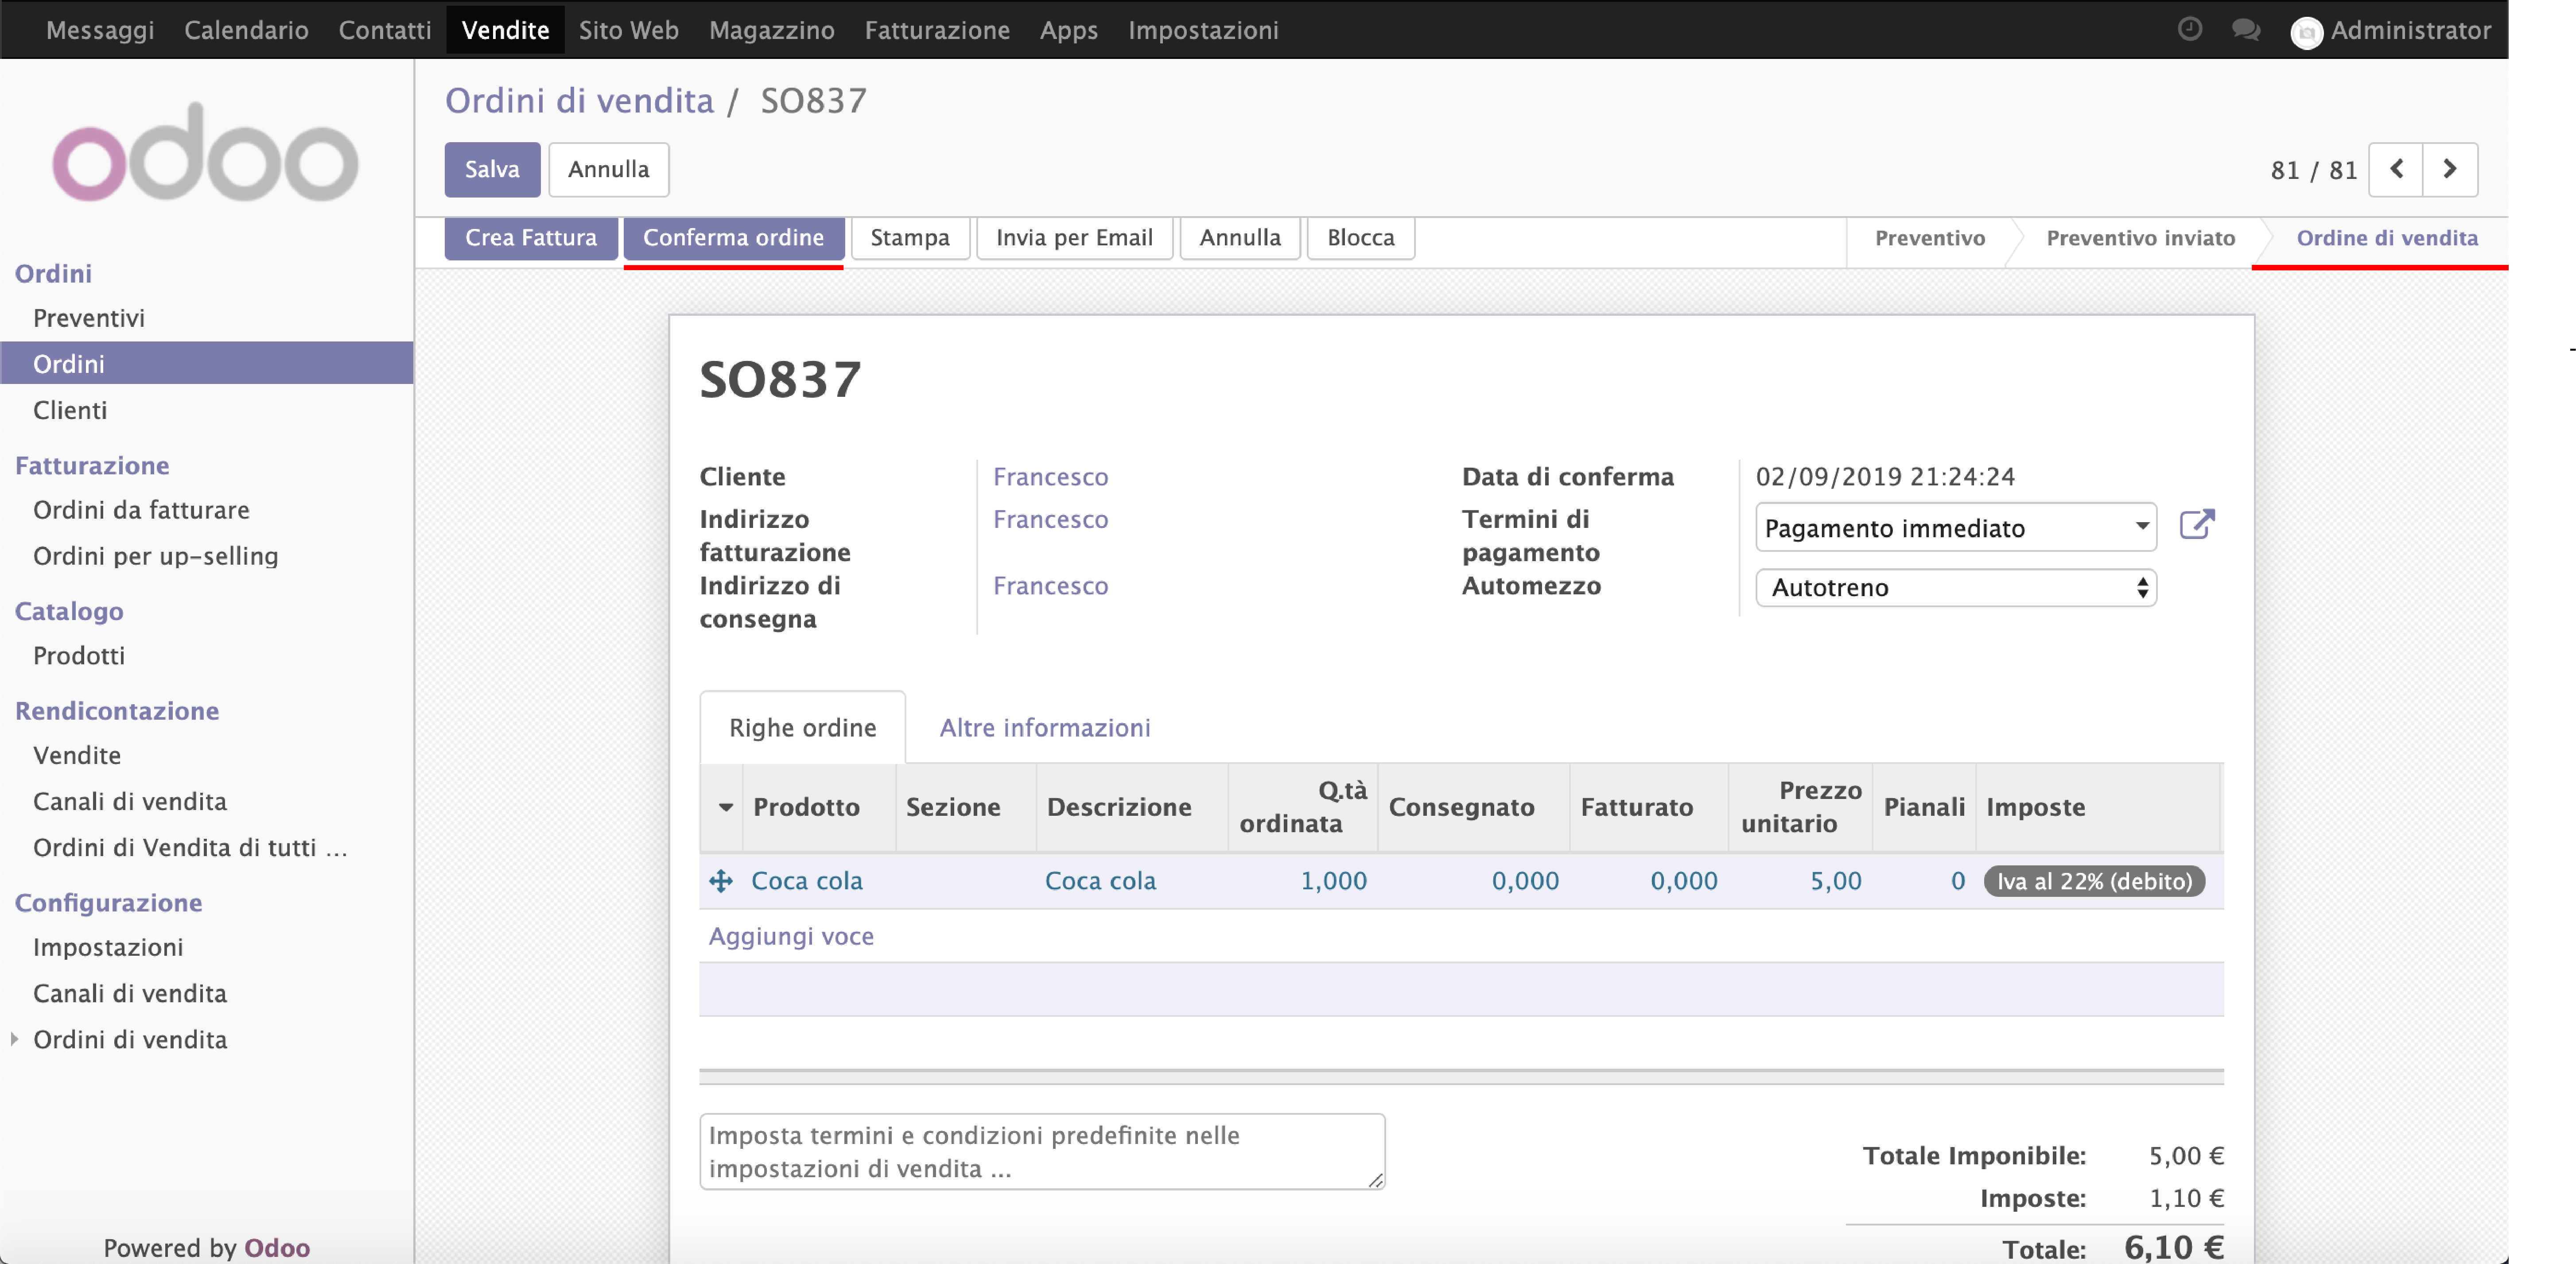
\includegraphics[scale=0.3]{figures/first_test}
		\caption[Test senza errori]{Test senza errori}
		\label{fig:first_test}
	\end{center}
\end{figure}

Invece, se al termine della procedura di compilazione dei campi vado a modificare il 'Prezzo unitario' (prezzo fisso del prodotto), e faccio click su 'Conferma ordine', verrà visualizzato il popup d'errore.
In questo caso abbiamo modificato lo stesso prodotto inserito precedentemente che costa € 5,00 con € 15,00. 
Una volta che si da l'ok al popup la fattura va nello stato 'Limite di Credito', dove non è più possibile modificarla.


\begin{figure}[H]
	\begin{center} 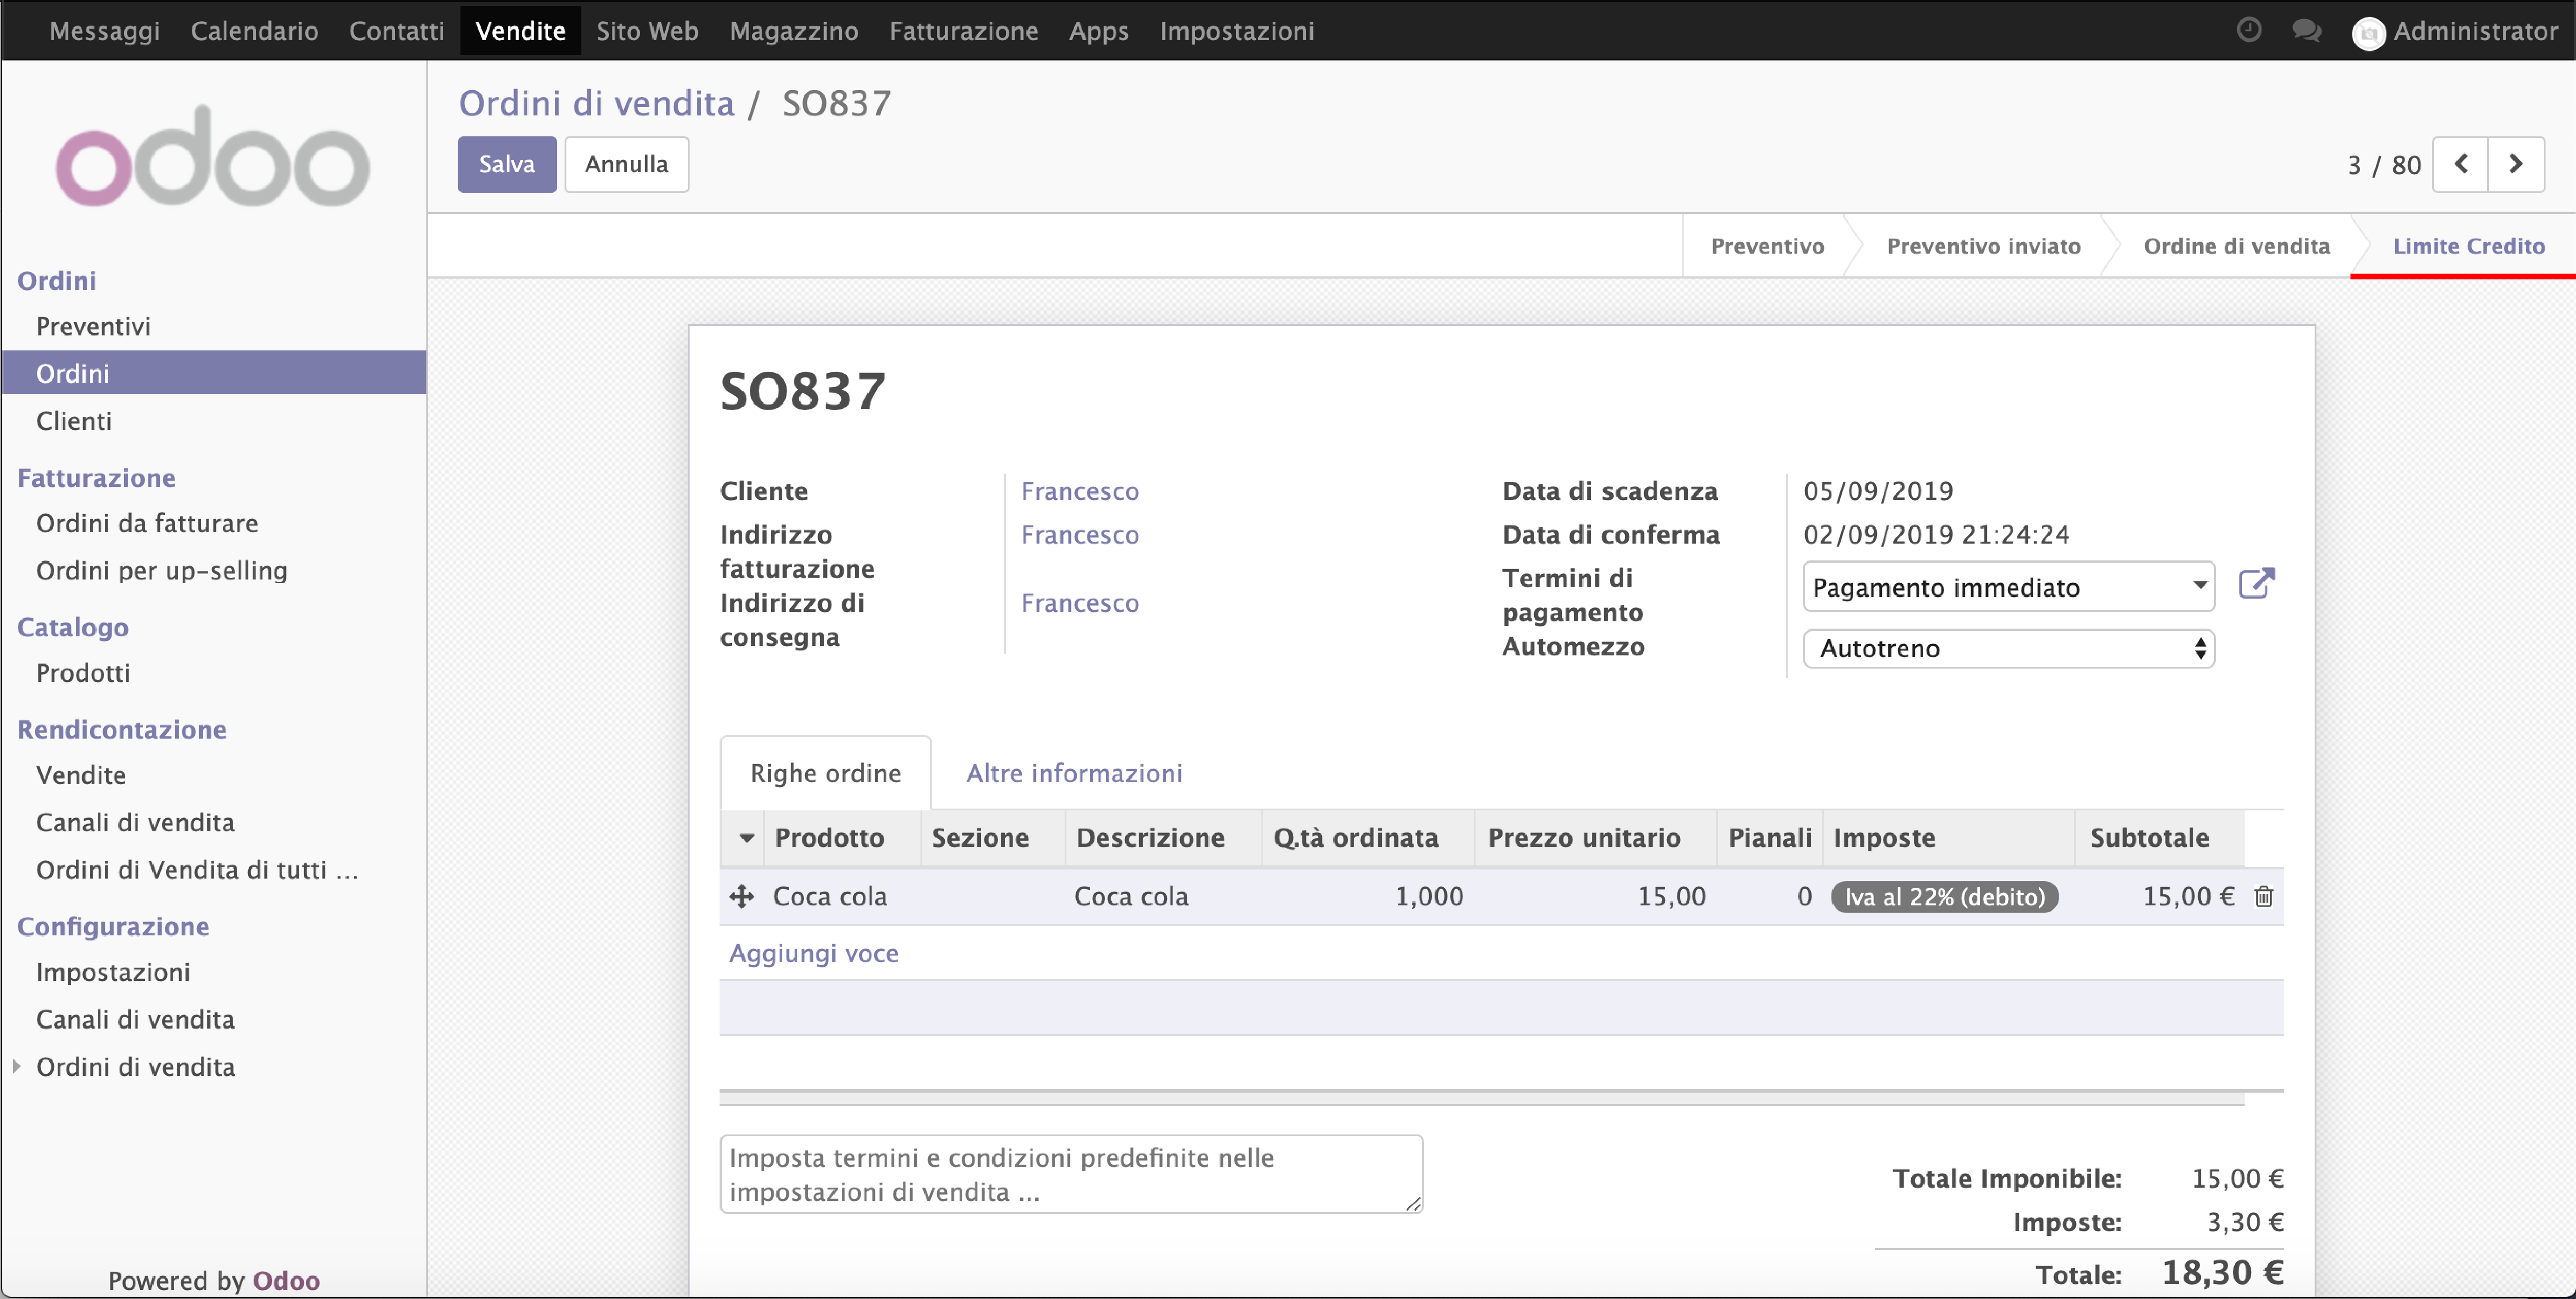
\includegraphics[scale=0.3]{figures/second_test}
		\caption[Test limite di credito]{Test limite di credito}
		\label{fig:second_test}
	\end{center}
\end{figure}

Per quanto riguarda il Blocco Scaduto, stiamo confermando un ordine con una data di scadenza antecedente a quella attuale, vuol dire che l'ordine di vendita è già scaduto.

\vspace*{0.5cm}
Per effettuare questo Test, abbiamo creato un 'Ordine di Vendita' ed abbiamo compilato i seguenti campi :

\begin{itemize}
	\item Cliente;
	\item Indirizzo di fatturazione;
	\item Indirizzo di consegna;
	\item Data di scadenza (antecedente alla data odierna);
	\item Termini di pagamento;
	\item Automezzo (selezione fra : Autotreno e Motrice);
	\item Seleziono un prodotto su Righe Ordine (tra quelli esistenti)
\end{itemize}

A questo punto, si fa un click sul pulsante 'Conferma ordine', si visualizzerà il popup di errore.
Una volta che si da l'ok al popup la fattura va nello stato 'Blocco Stato', dove non è più possibile modificarla.


\begin{figure}[H]
	\begin{center} 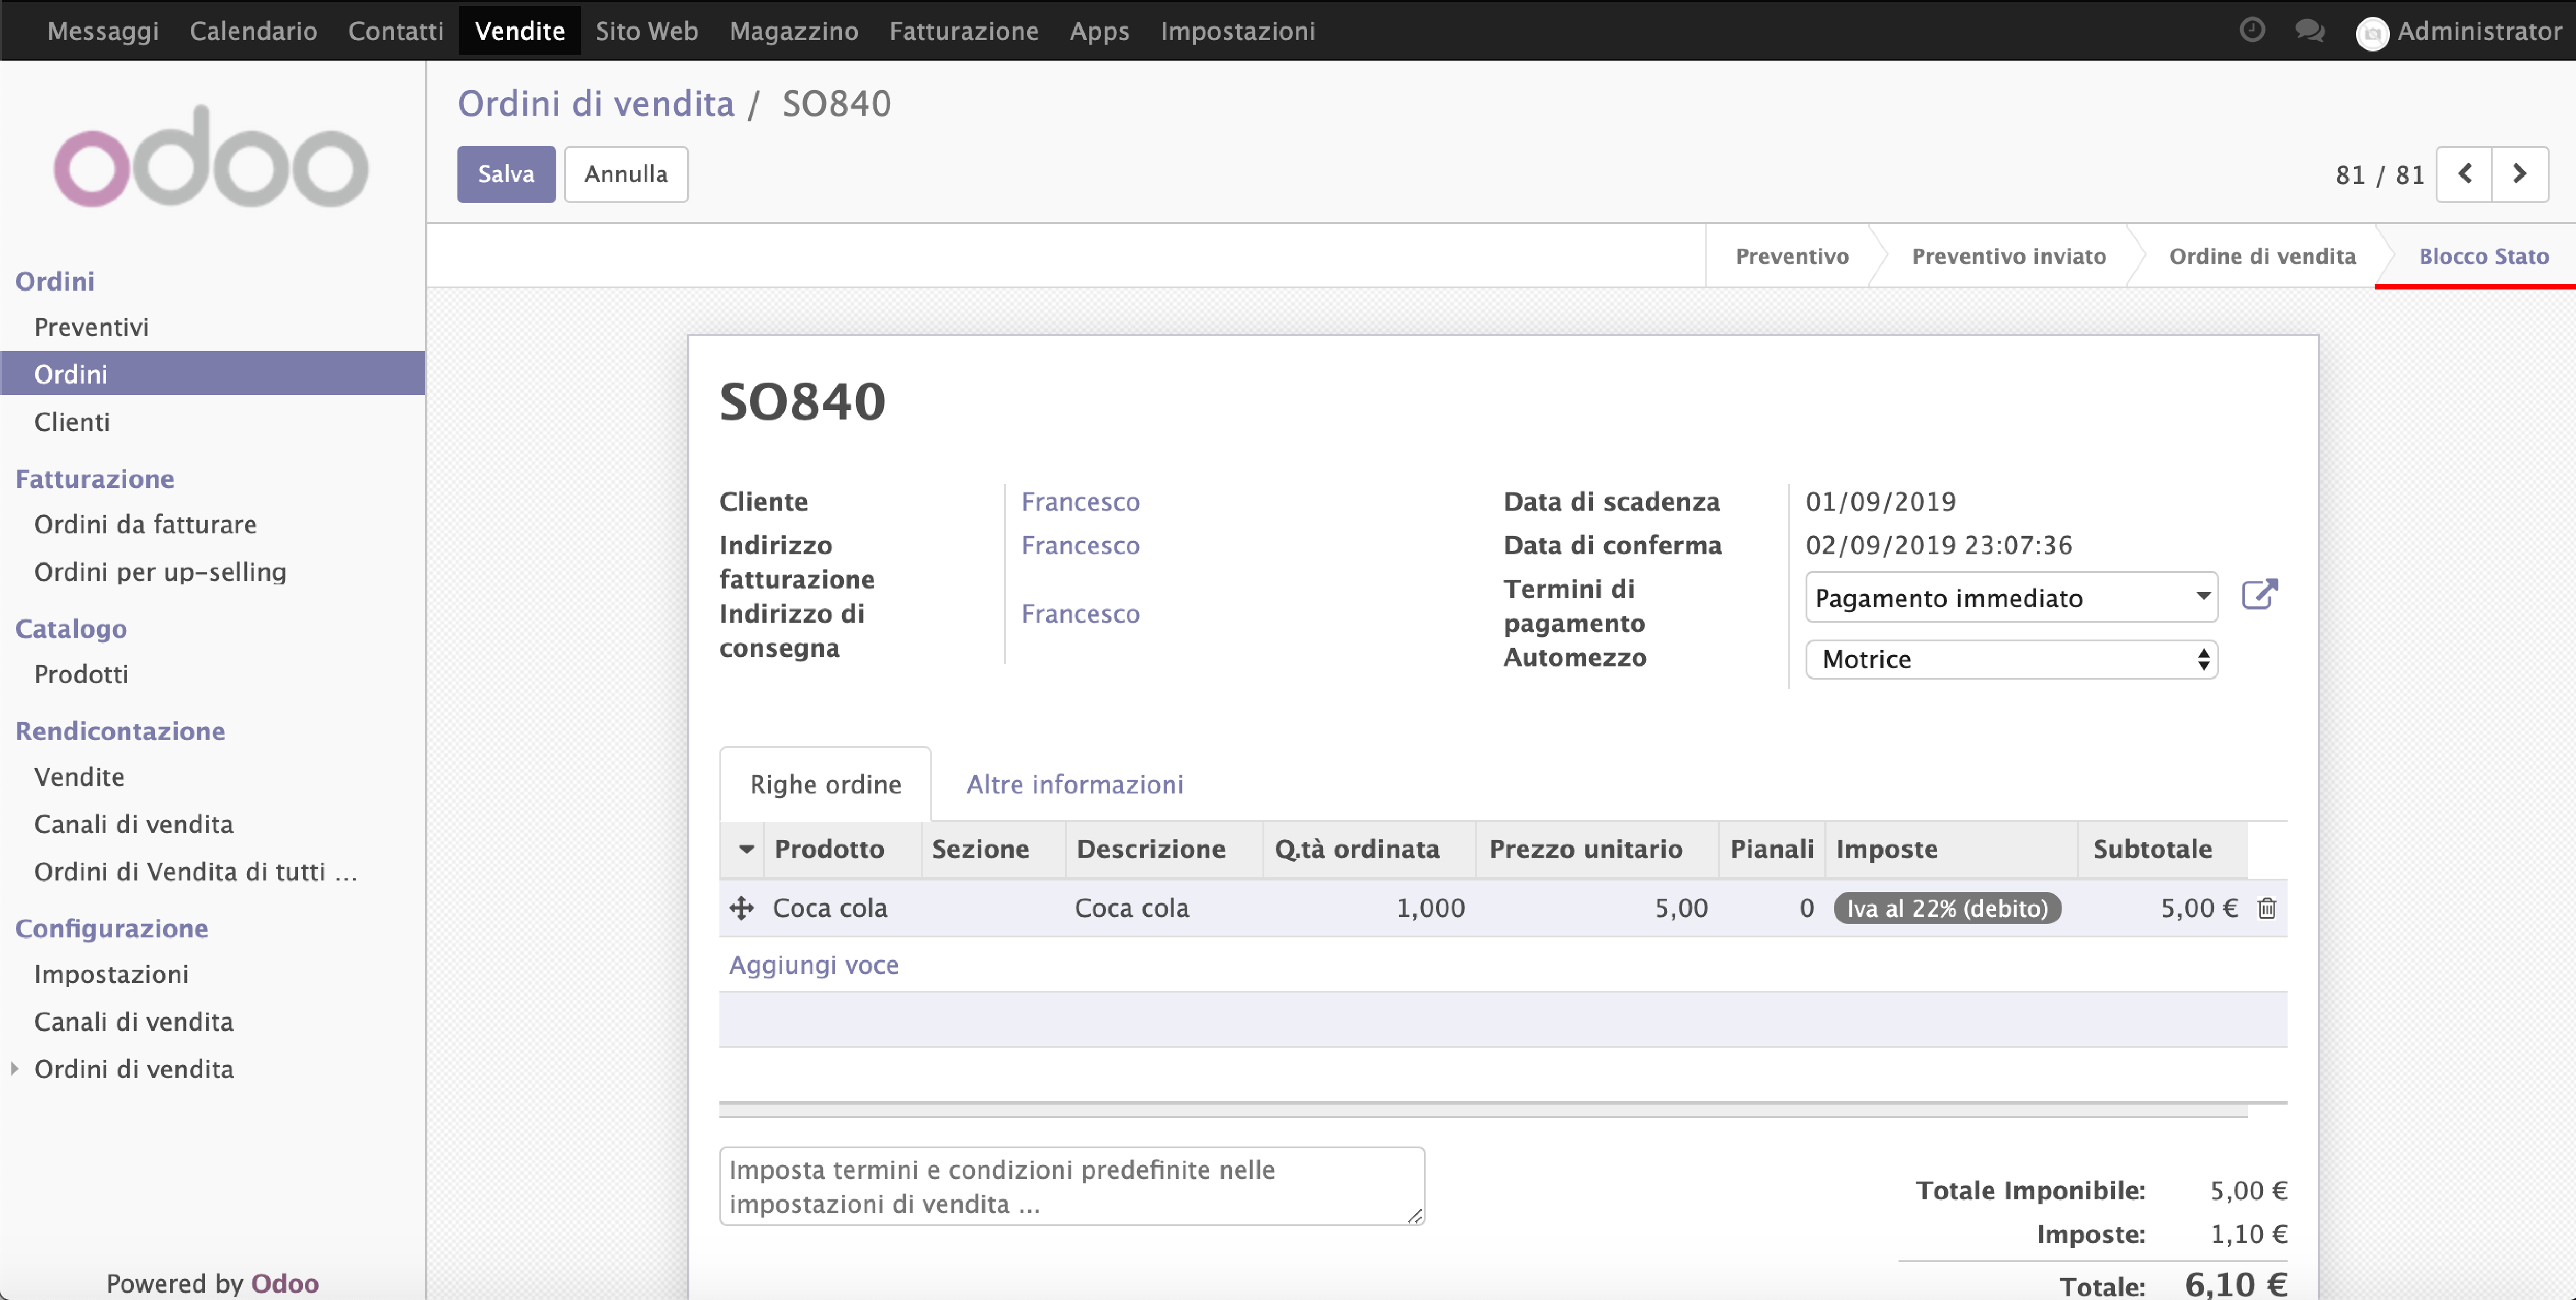
\includegraphics[scale=0.3]{figures/third_test}
		\caption[Test blocco scaduto]{Test blocco scaduto}
		\label{fig:third_test}
	\end{center}
\end{figure}

\subsection{Canali di Vendita}

Su questo modulo, abbiamo verificato che ll campo 'Codice canale di vendita' viene valorizzato con il campo 'Codice canale' + nome del 'Canale di vendita'.

\vspace*{0.5cm}
Per effettuare questo Test, abbiamo creato un 'Canale di Vendita' ed abbiamo compilato i seguenti campi :
\begin{itemize}
\item Canale di Vendita;
\item Codice canale;
\end{itemize}
\newpage
In automatico il campo 'Codice canale di vendita' (che è \glo{readonly}), verrà valorizzato correttamente.
  
\begin{figure}[H]
	\begin{center} 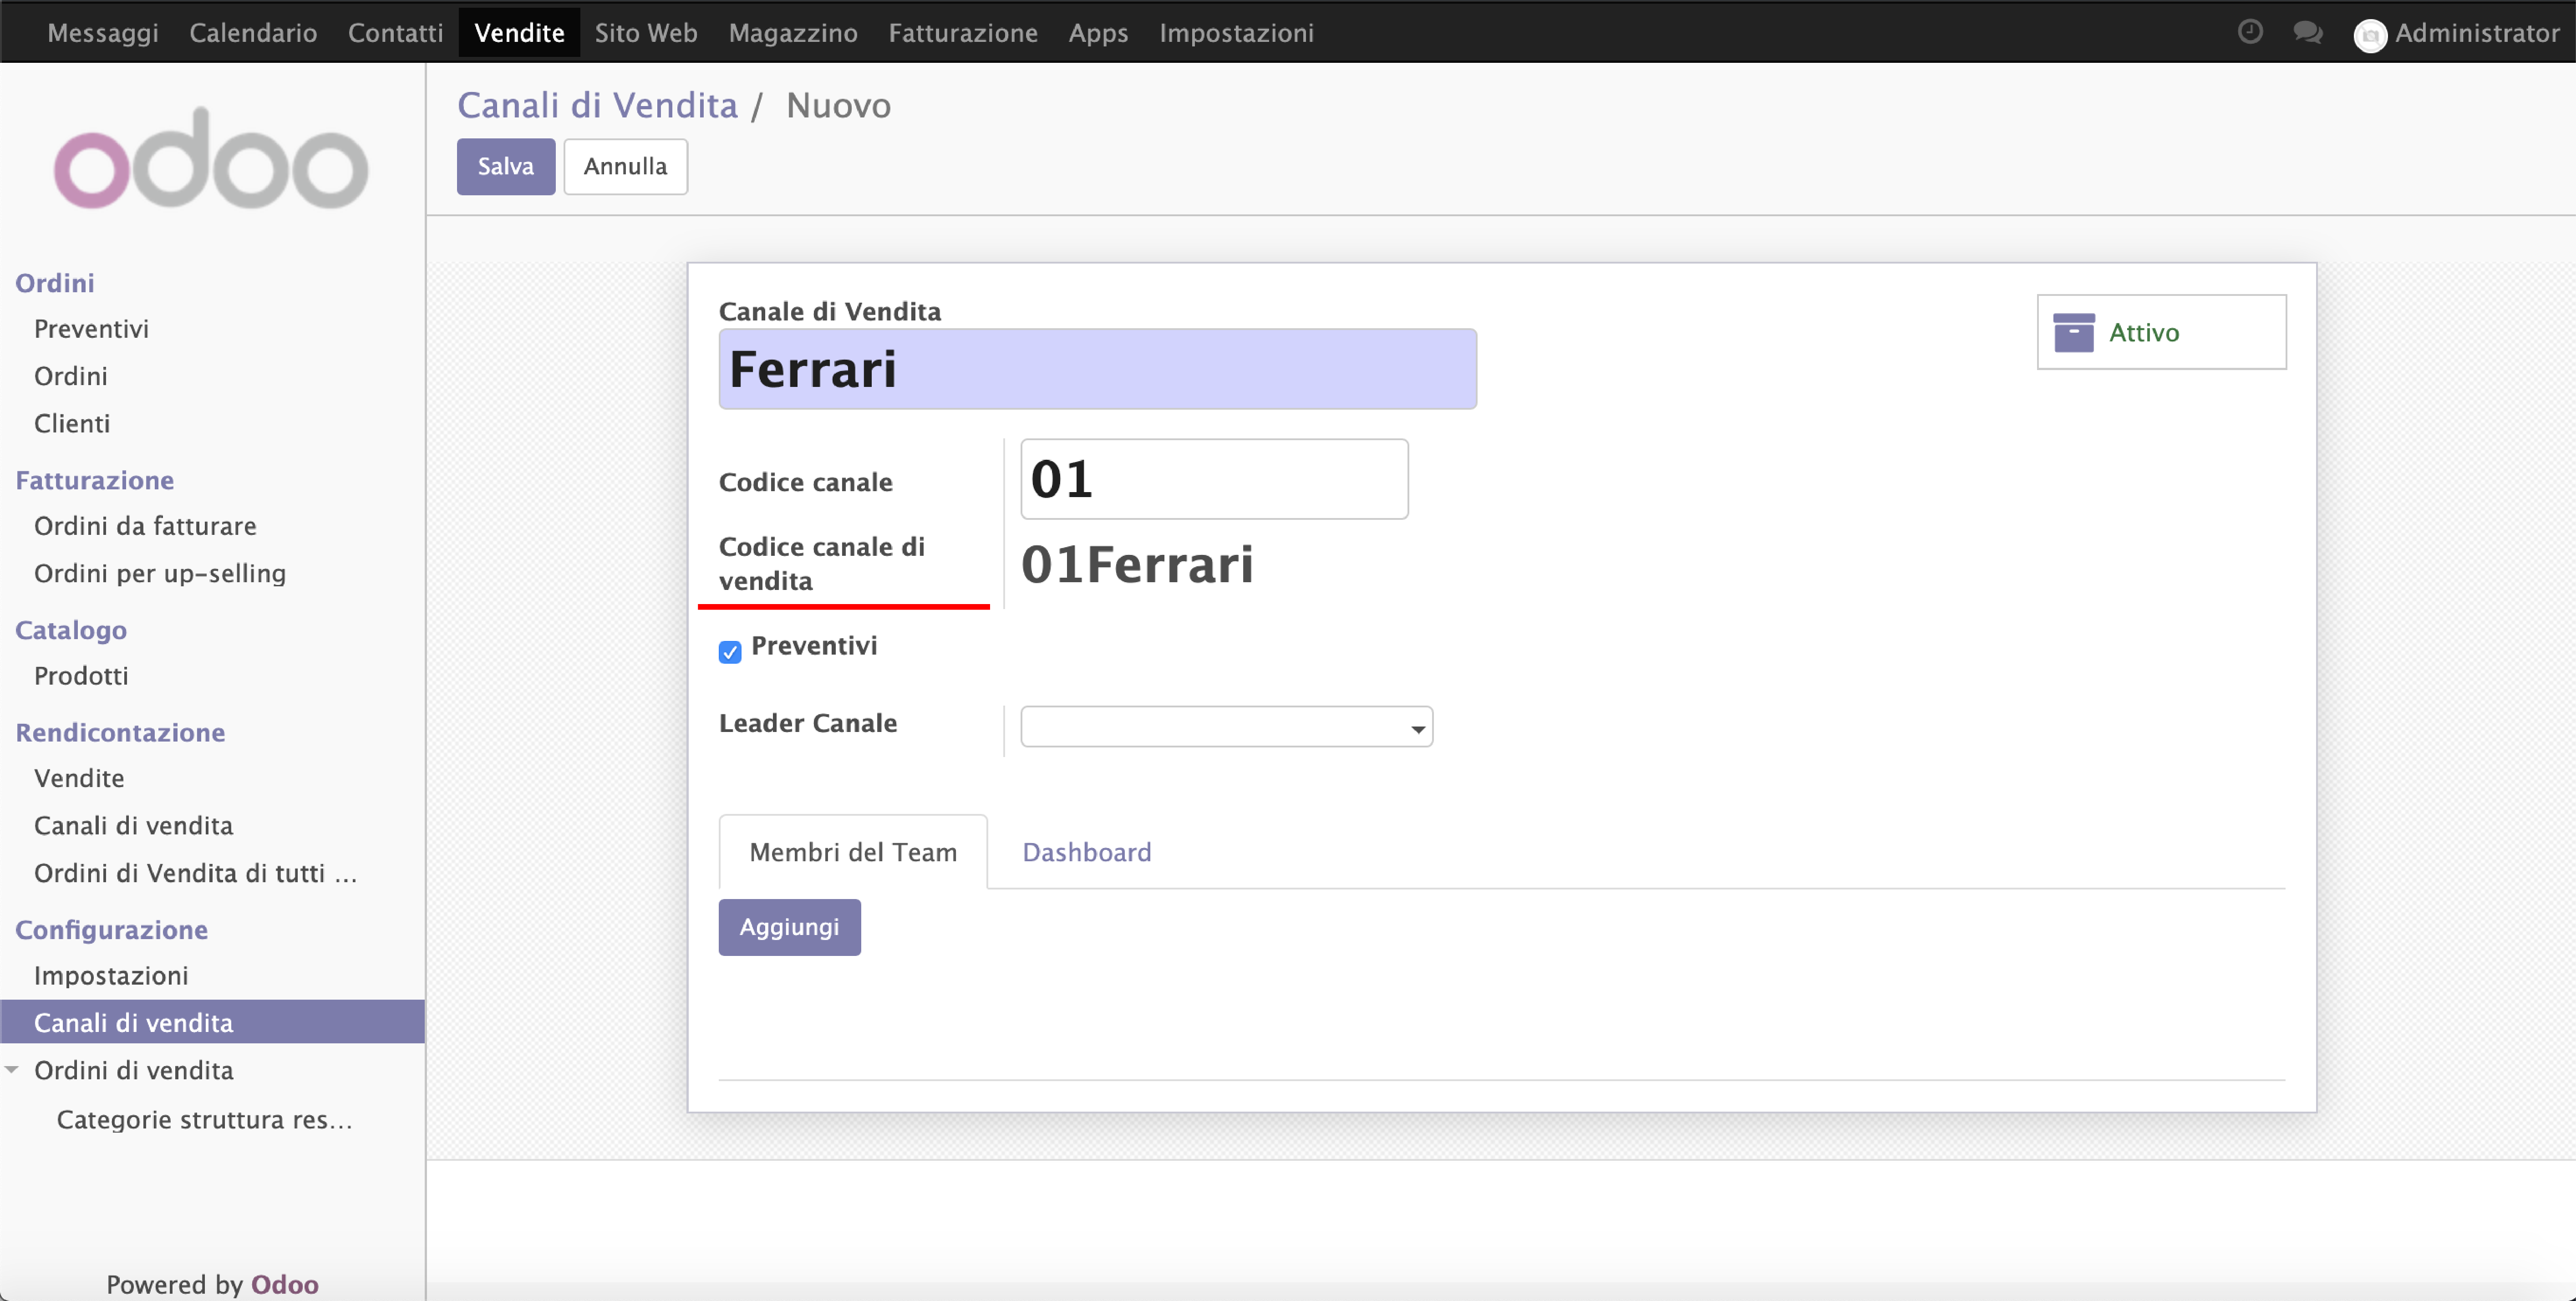
\includegraphics[scale=0.3]{figures/fourth_test}
		\caption[Test canale di vendita]{Test canale di vendita}
		\label{fig:fourth_test}
	\end{center}
\end{figure}


\subsection{Gestione imballi}

Per effettuare questo Test, abbiamo creato un 'Ordine di vendita' ed abbiamo compilato i seguenti campi :
\begin{itemize}
	\item Cliente;
	\item Indirizzo di fatturazione;
	\item Indirizzo di consegna;
	\item Data di scadenza (successiva alla data odierna);
	\item Termini di pagamento;
	\item Automezzo (selezione fra : Autotreno e Motrice);
	\item Seleziono 'Aggiungi voce' su Righe Ordine (per selezionare un prodotto)
\end{itemize}

Quando abbiamo fatto click sul campo 'Aggiungi voce', che mi permette di inserire un prodotto, visualizzerò un altro form dove compilerò i seguenti campi:
\begin{itemize}
\item Prodotto;
\item Sezione;
\item Quantità ordinata (in questo esempio: 20);
\item Confezione;
\item Imposte (IVA facoltativa);
\item Tempo di consegna (giorni);
\end{itemize}

Come confezione abbiamo selezionato un esempio creato, di nome 'Tipo', che ha per 'Quantità per confezione'= 7 (denominatore).
\vspace*{1cm}
\begin{figure}[H]
	\begin{center} 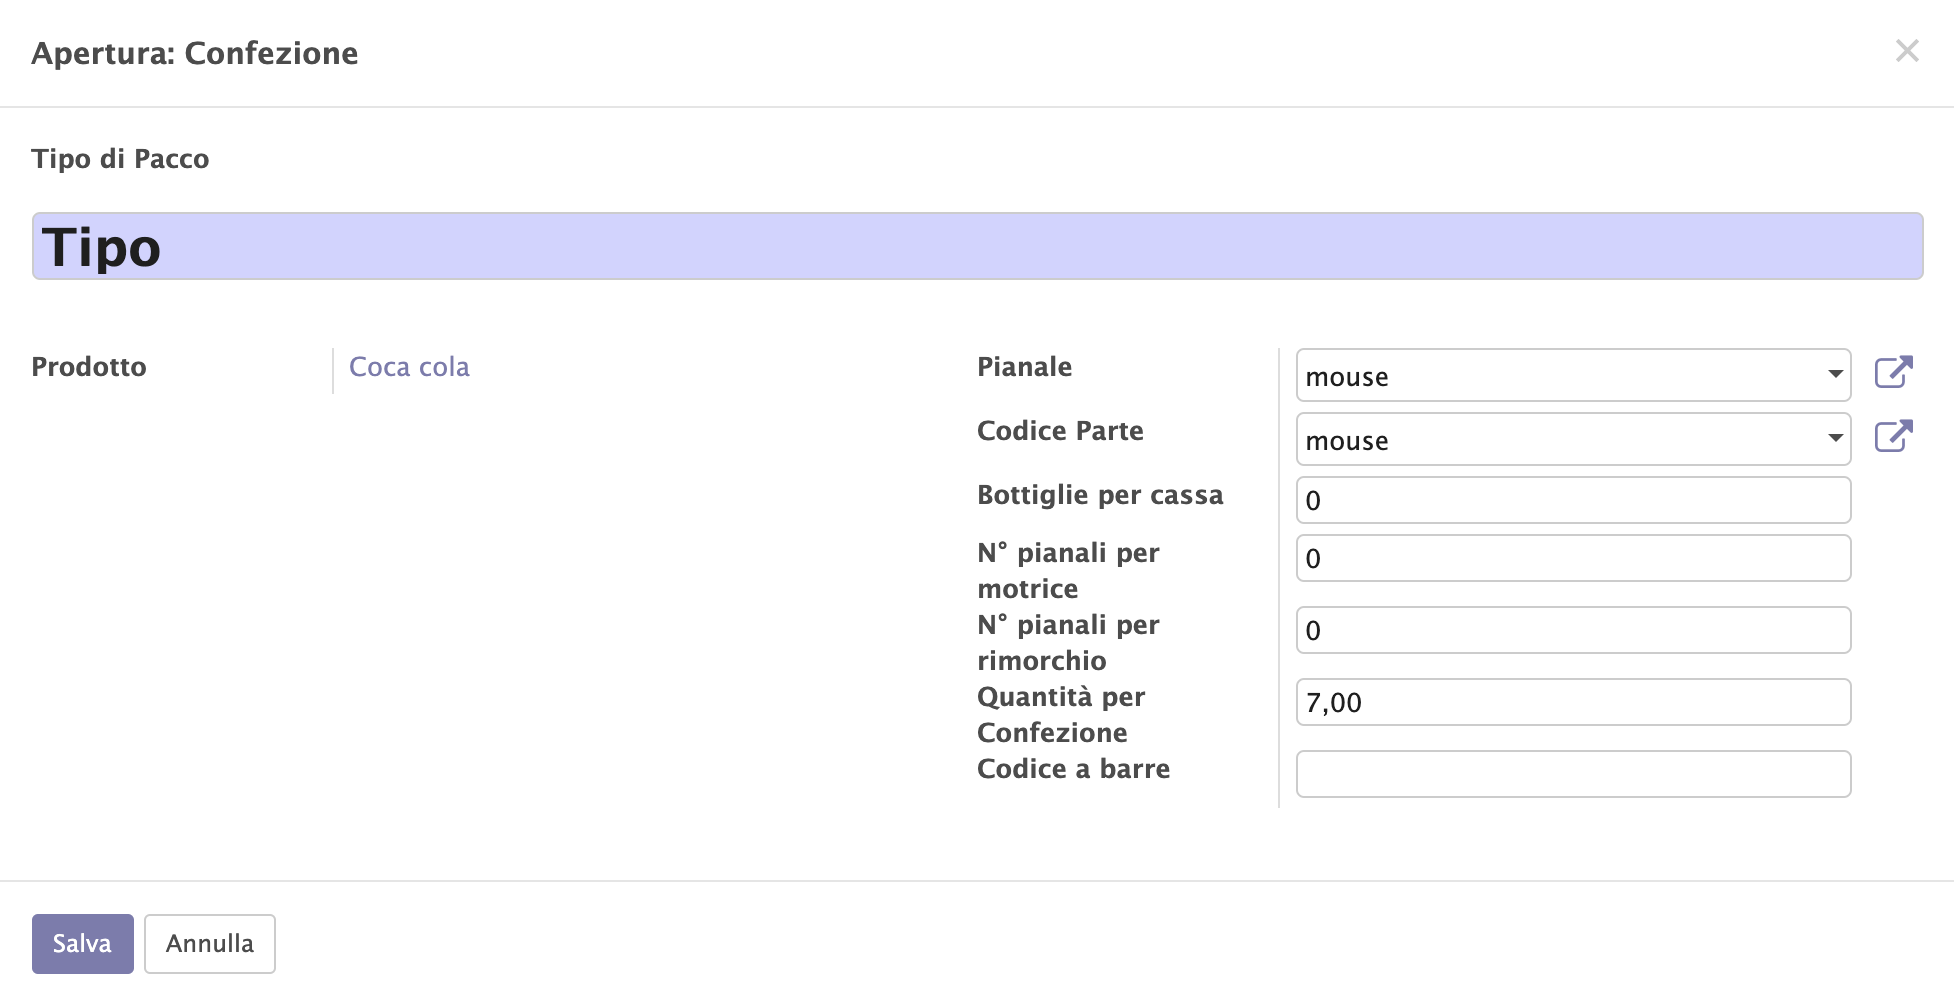
\includegraphics[scale=0.3]{figures/package}
		\caption[Esempio form confezione]{Esempio form confezione}
		\label{fig:package}
	\end{center}
\end{figure}

\newpage
A questo punto salviamo la confezione, il prodotto, e ritorniamo all'interfaccia di 'Ordine di vendita'.
Facciamo click su 'Conferma Ordine'. Come detto in precedenza, il campo 'Pianali' si compila automaticamente; è dato dal rapporto fra Quantità ordinata (20) / Quantità per confezione (7) = 2,85.\\
Il risultato è un numero decimale superiore all'unità, il valore, del campo 'Pianali', verrà approssimato per difetto all'intero più vicino.\\
( Risultato rapporto = 2,85 campo pianali = 2)

\begin{figure}[H]
	\begin{center} 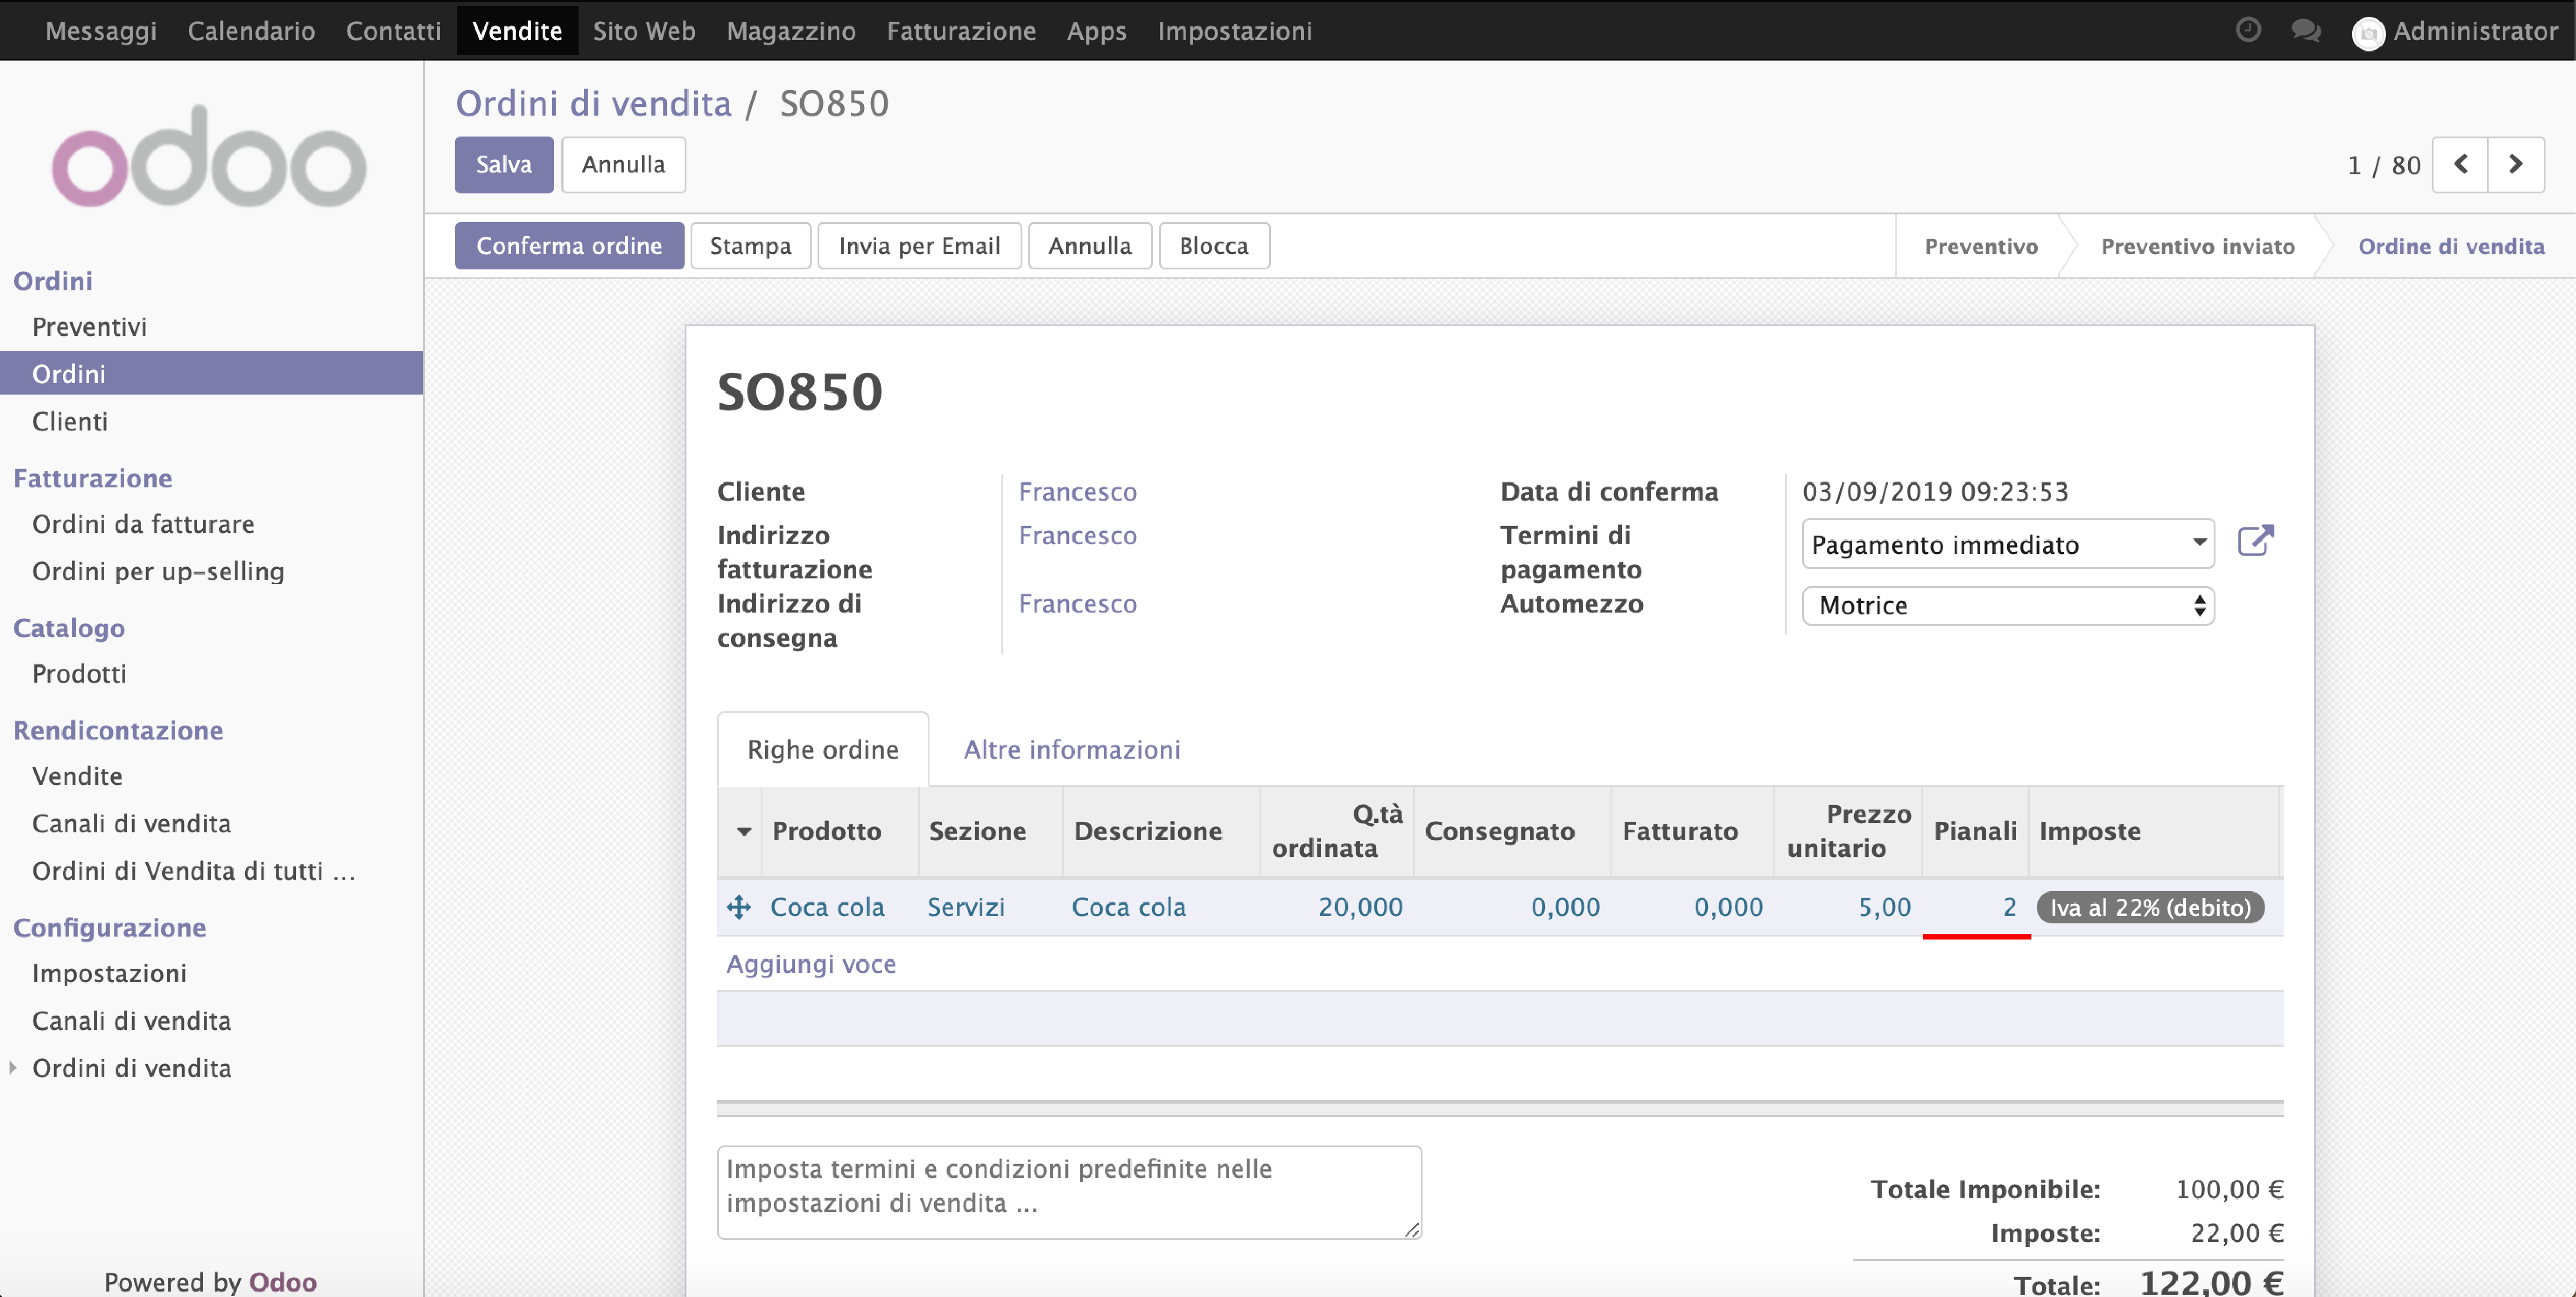
\includegraphics[scale=0.3]{figures/fifth_test}
		\caption[Primo Test campo 'Pianali']{Primo Test campo 'Pianali'}
		\label{fig:fifth_test}
	\end{center}
\end{figure}
\newpage
Se il rapporto da come risultato un numero intero, il sistema deve compilare il campo Pianali con il risultato del rapporto.
In questo caso abbiamo settato la Quantità ordinata (5) / Quantità per confezione (5) = 1.

( Risultato rapporto = 1 campo pianali = 1)
\begin{figure}[H]
	\begin{center} 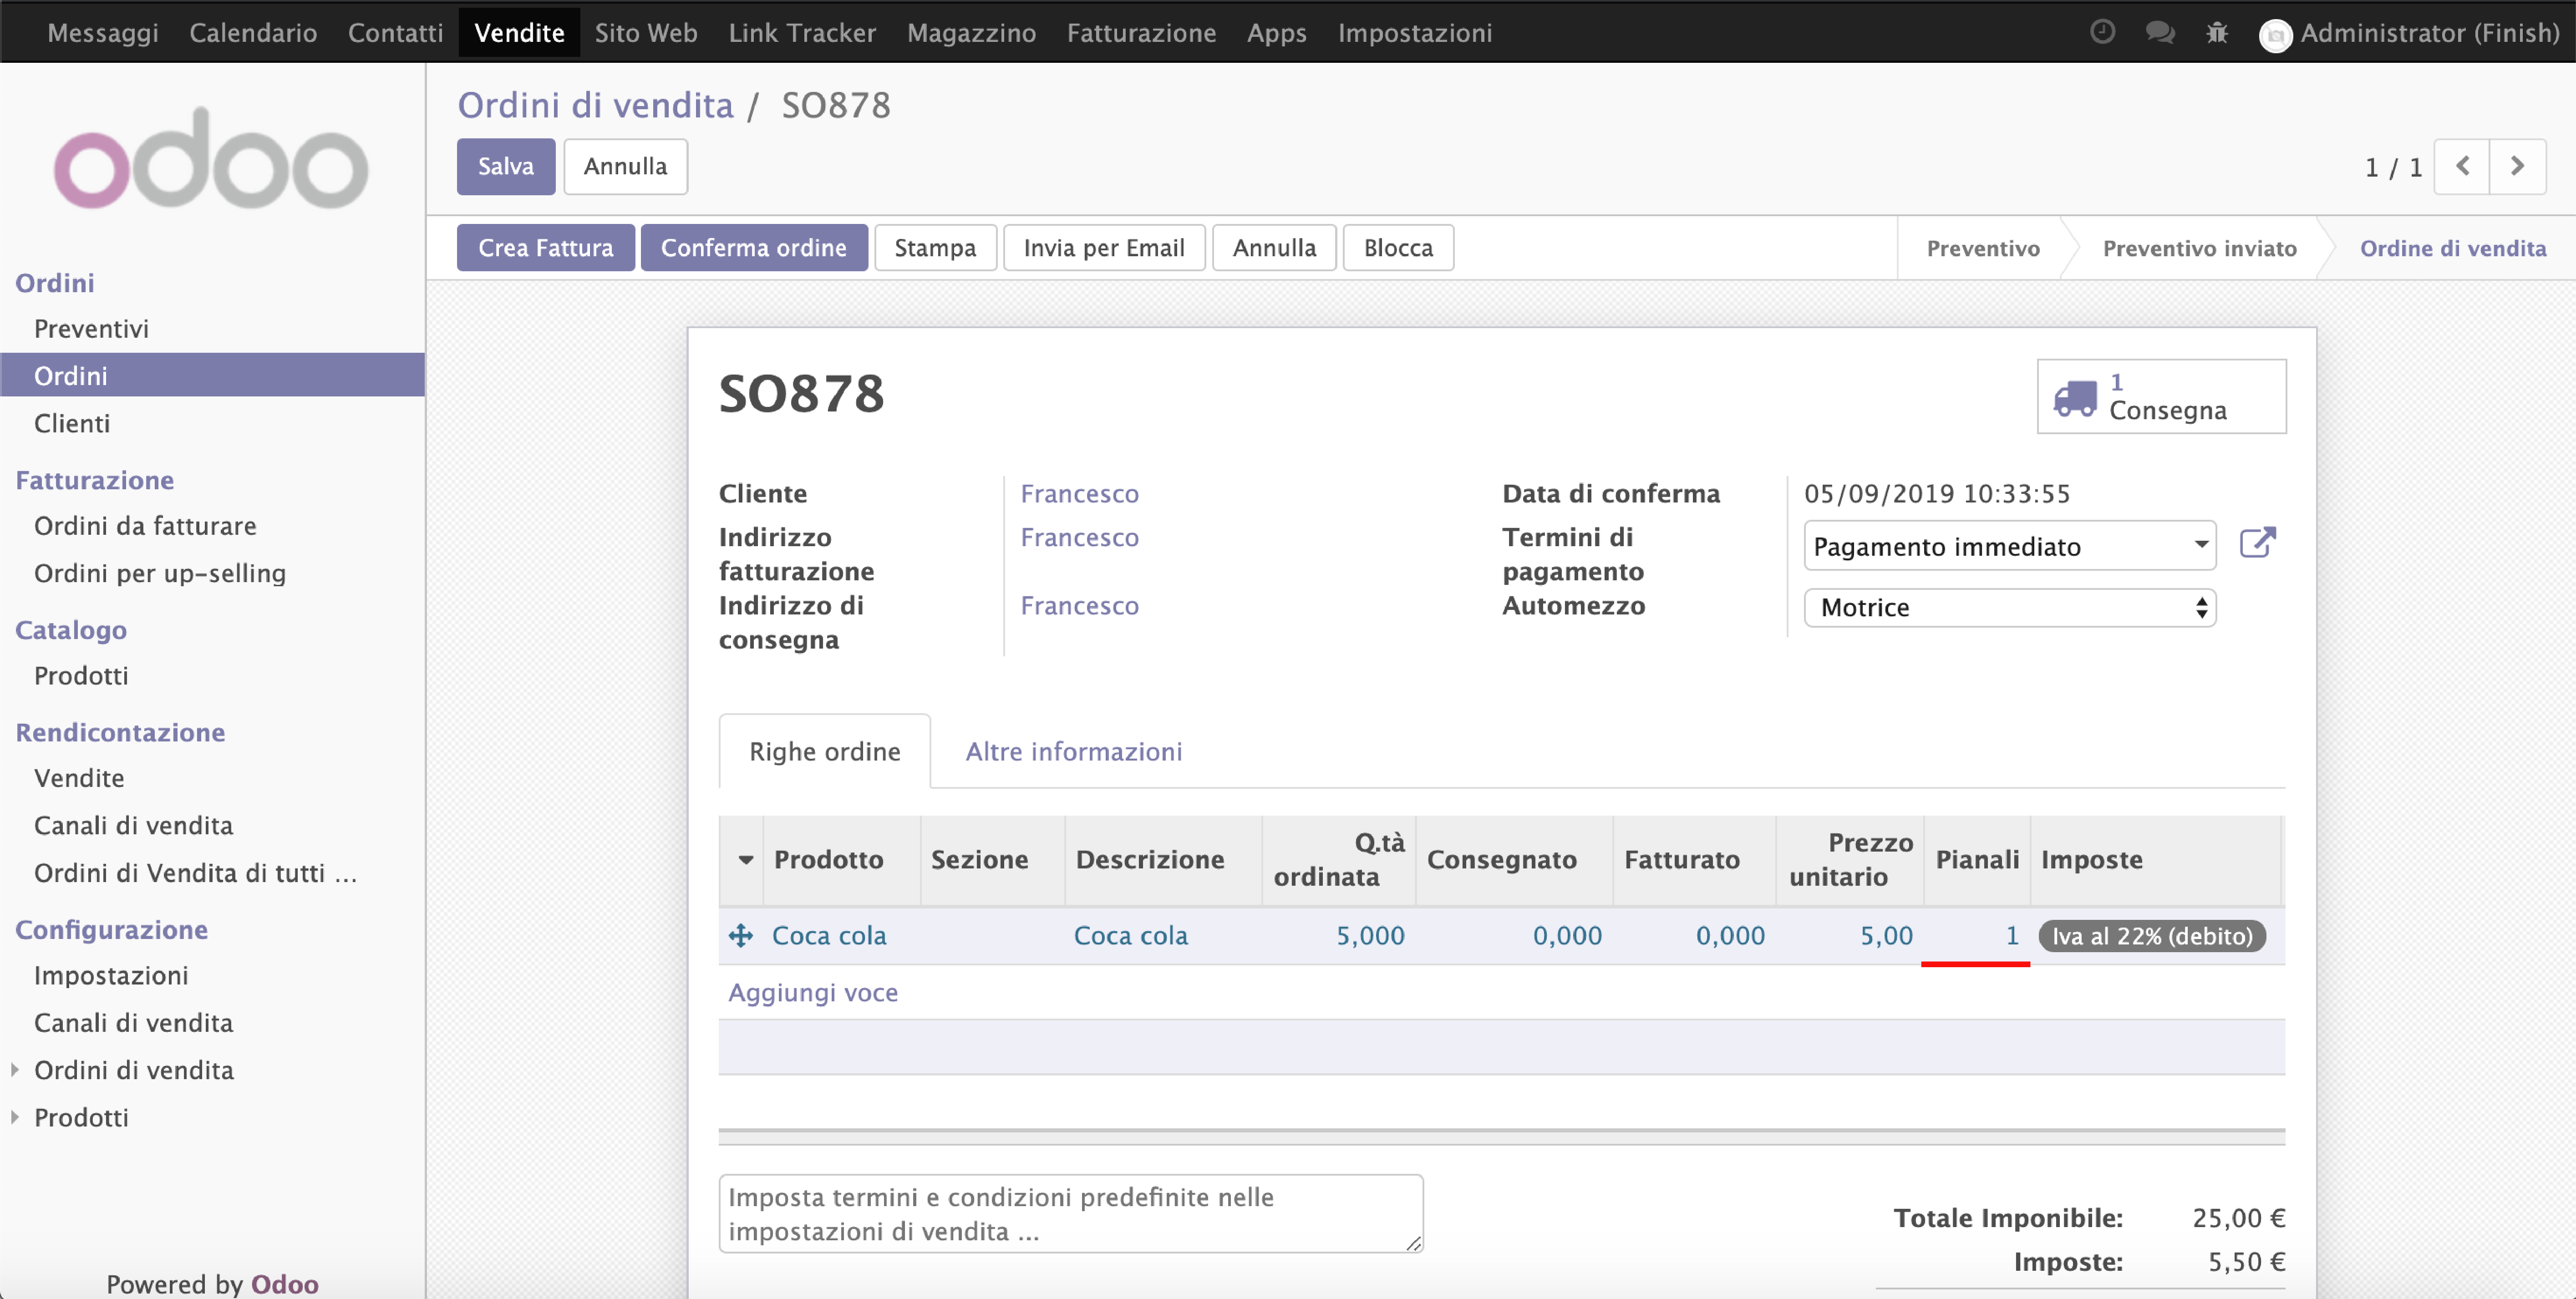
\includegraphics[scale=0.3]{figures/sixth_test}
		\caption[Secondo Test campo 'Pianali']{Secondo Test campo 'Pianali'}
		\label{fig:sixth_test}
	\end{center}
\end{figure}
\newpage
Se il rapporto da come risultato un numero decimale inferiore all'unità il campo Pianali va settato a null.
In questo caso abbiamo settato la Quantità ordinata (1) / Quantità per confezione (5) = 0,2.\\
( Risultato rapporto = 0,2 campo pianali = 0)

\begin{figure}[H]
	\begin{center} 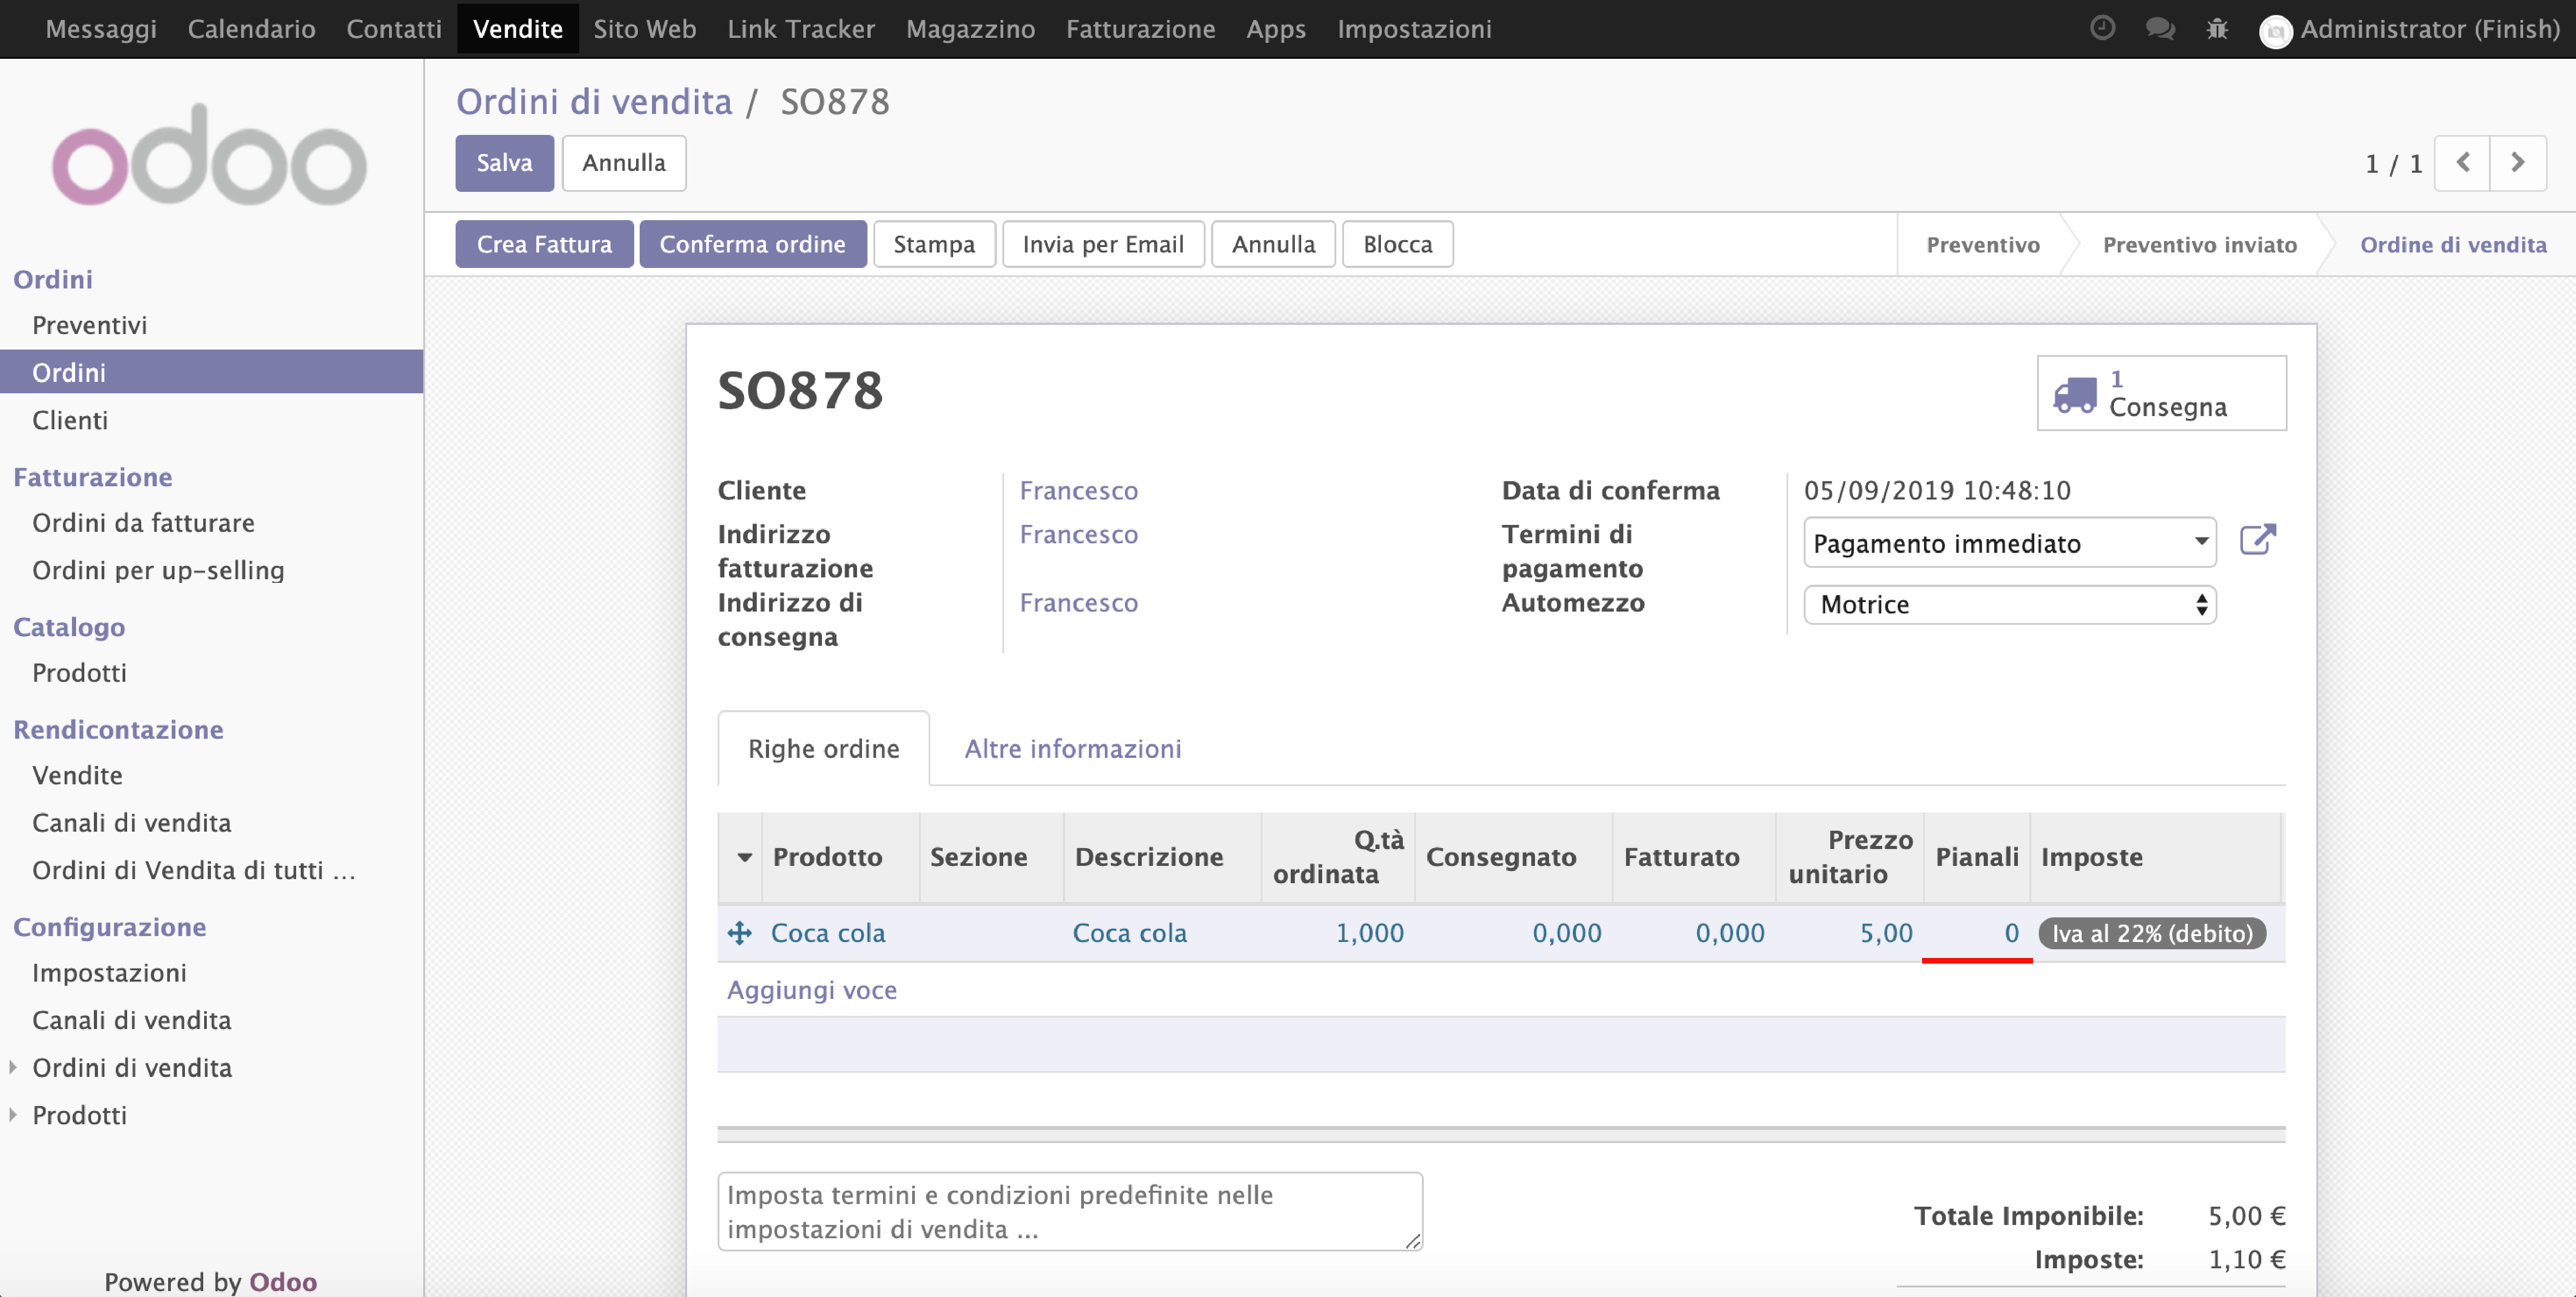
\includegraphics[scale=0.3]{figures/seventh_test}
		\caption[Terzo Test campo 'Pianali']{Terzo Test campo 'Pianali'}
		\label{fig:seventh_test}
	\end{center}
\end{figure}

\newpage
Infine al salvataggio di un ordine di vendita abbiamo creato un test per controllare che all'inserimento di uno stesso prodotto, occorre rendere unica la \textit{line} aggiornandone solo la quantità.

\begin{figure}[H]
	\begin{center} 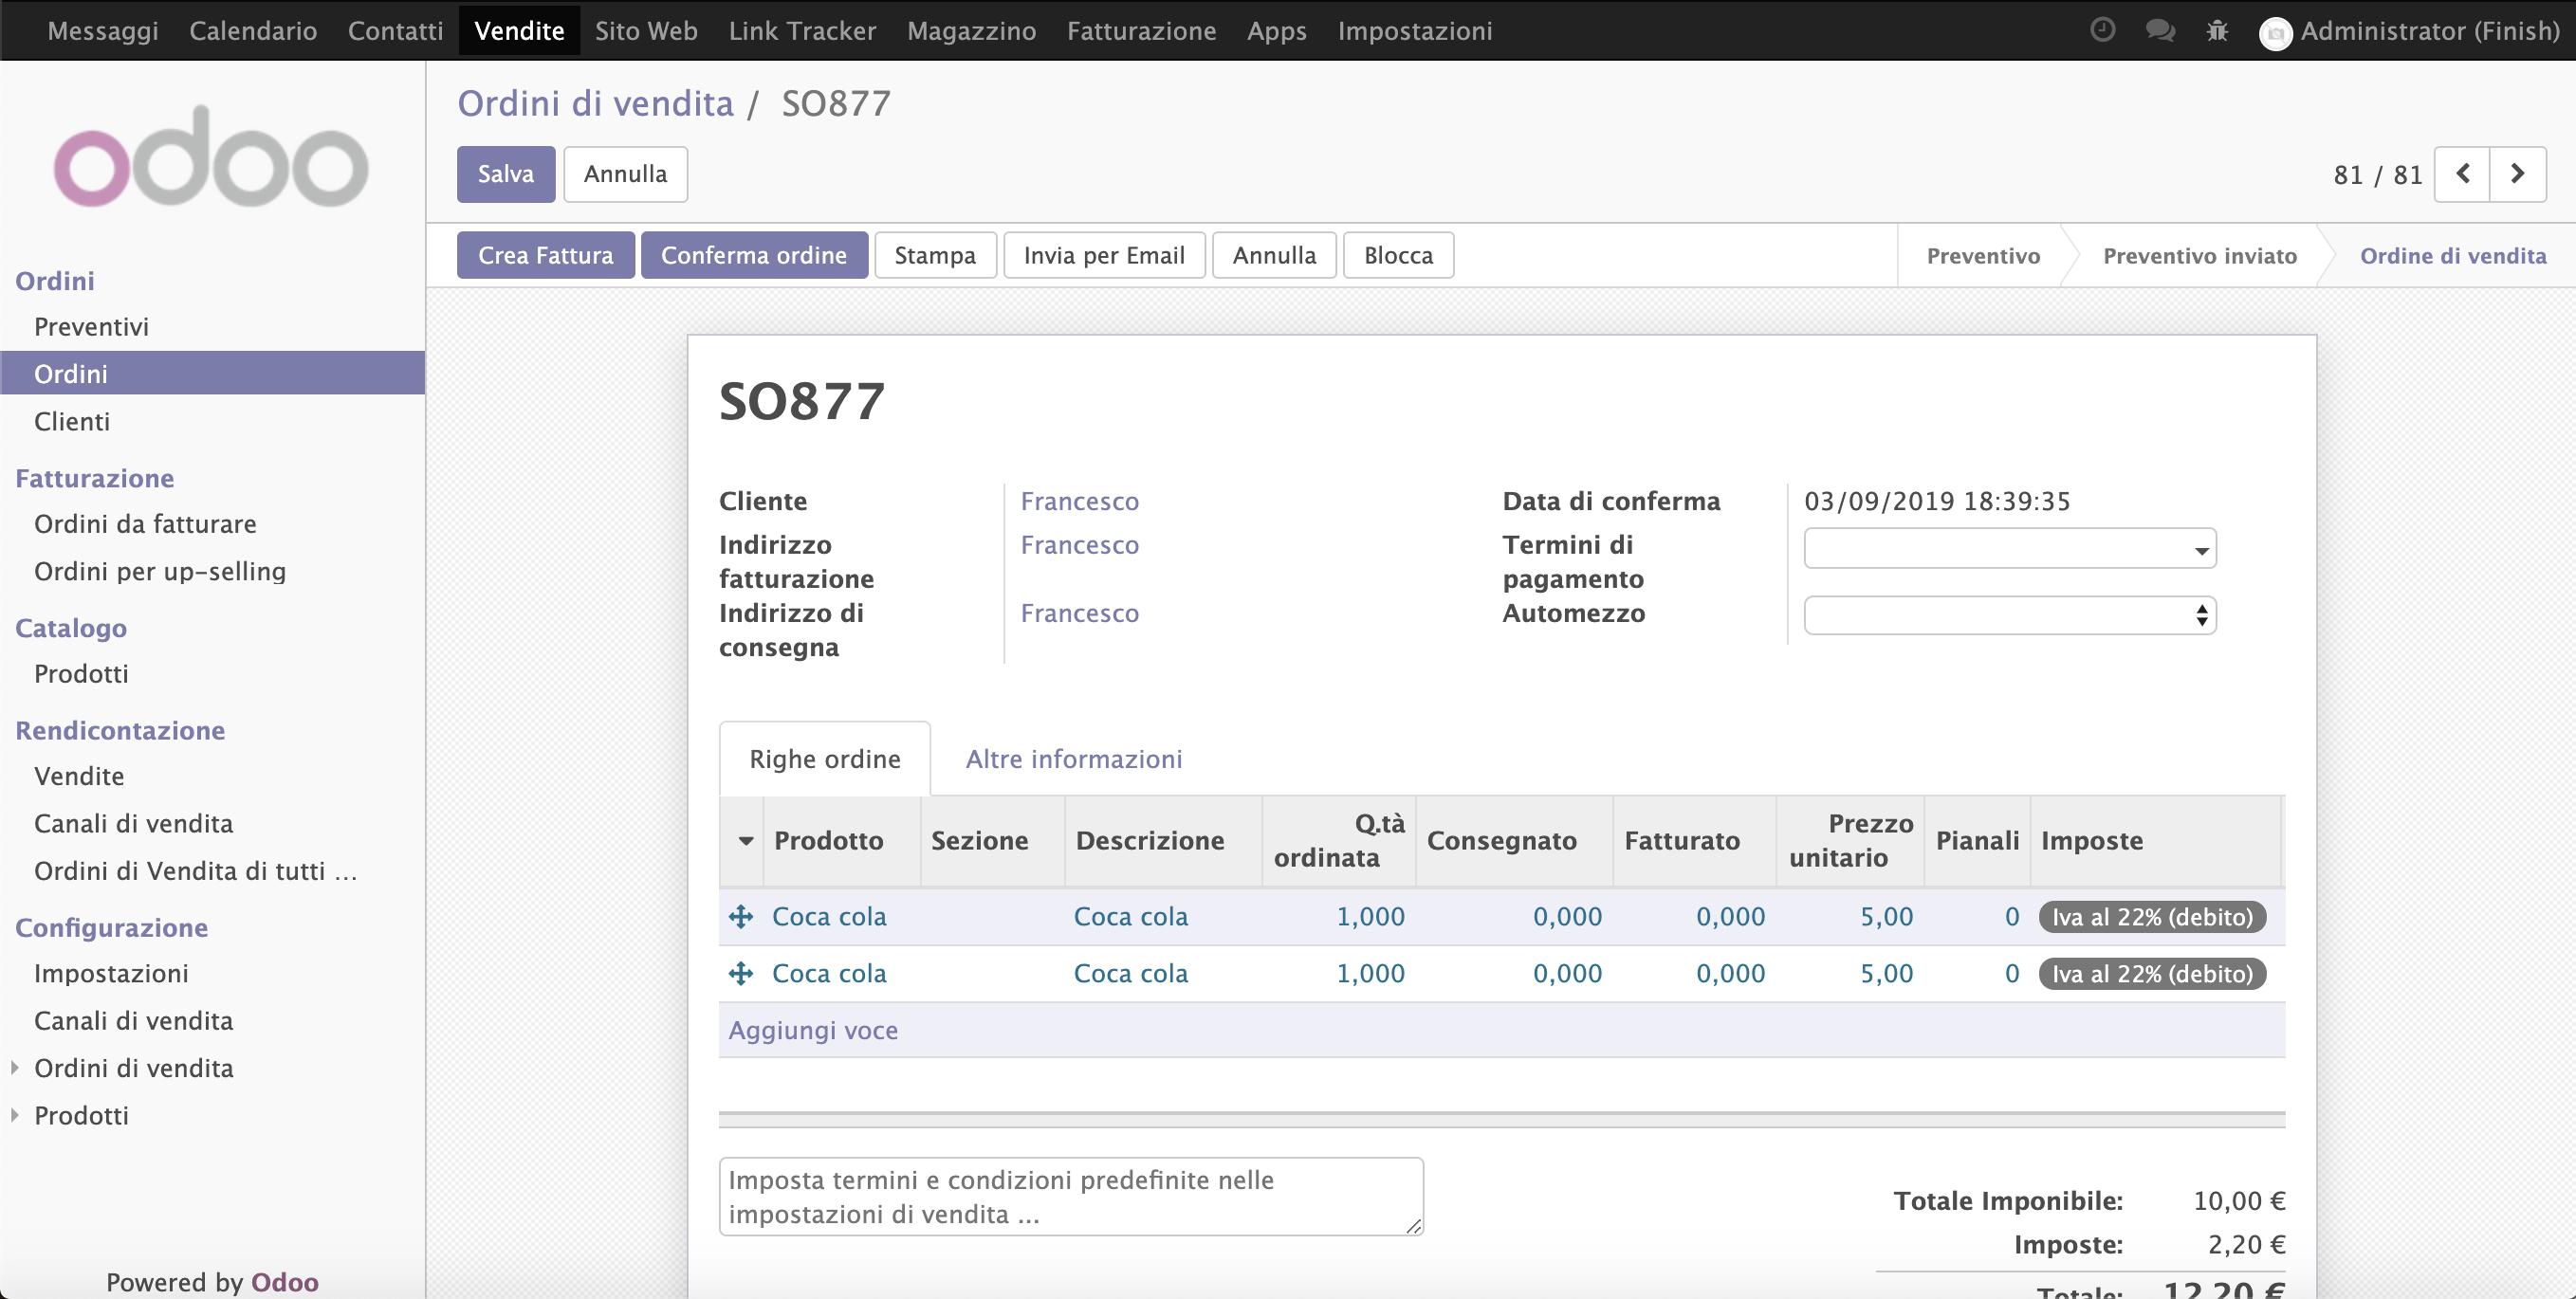
\includegraphics[scale=0.3]{figures/ctrl_1}
		\caption[Inserimento di uno stesso prodotto]{Inserimento di uno stesso prodotto}
		\label{fig:ctrl_1}
	\end{center}
\end{figure}

\begin{figure}[H]
	\begin{center} 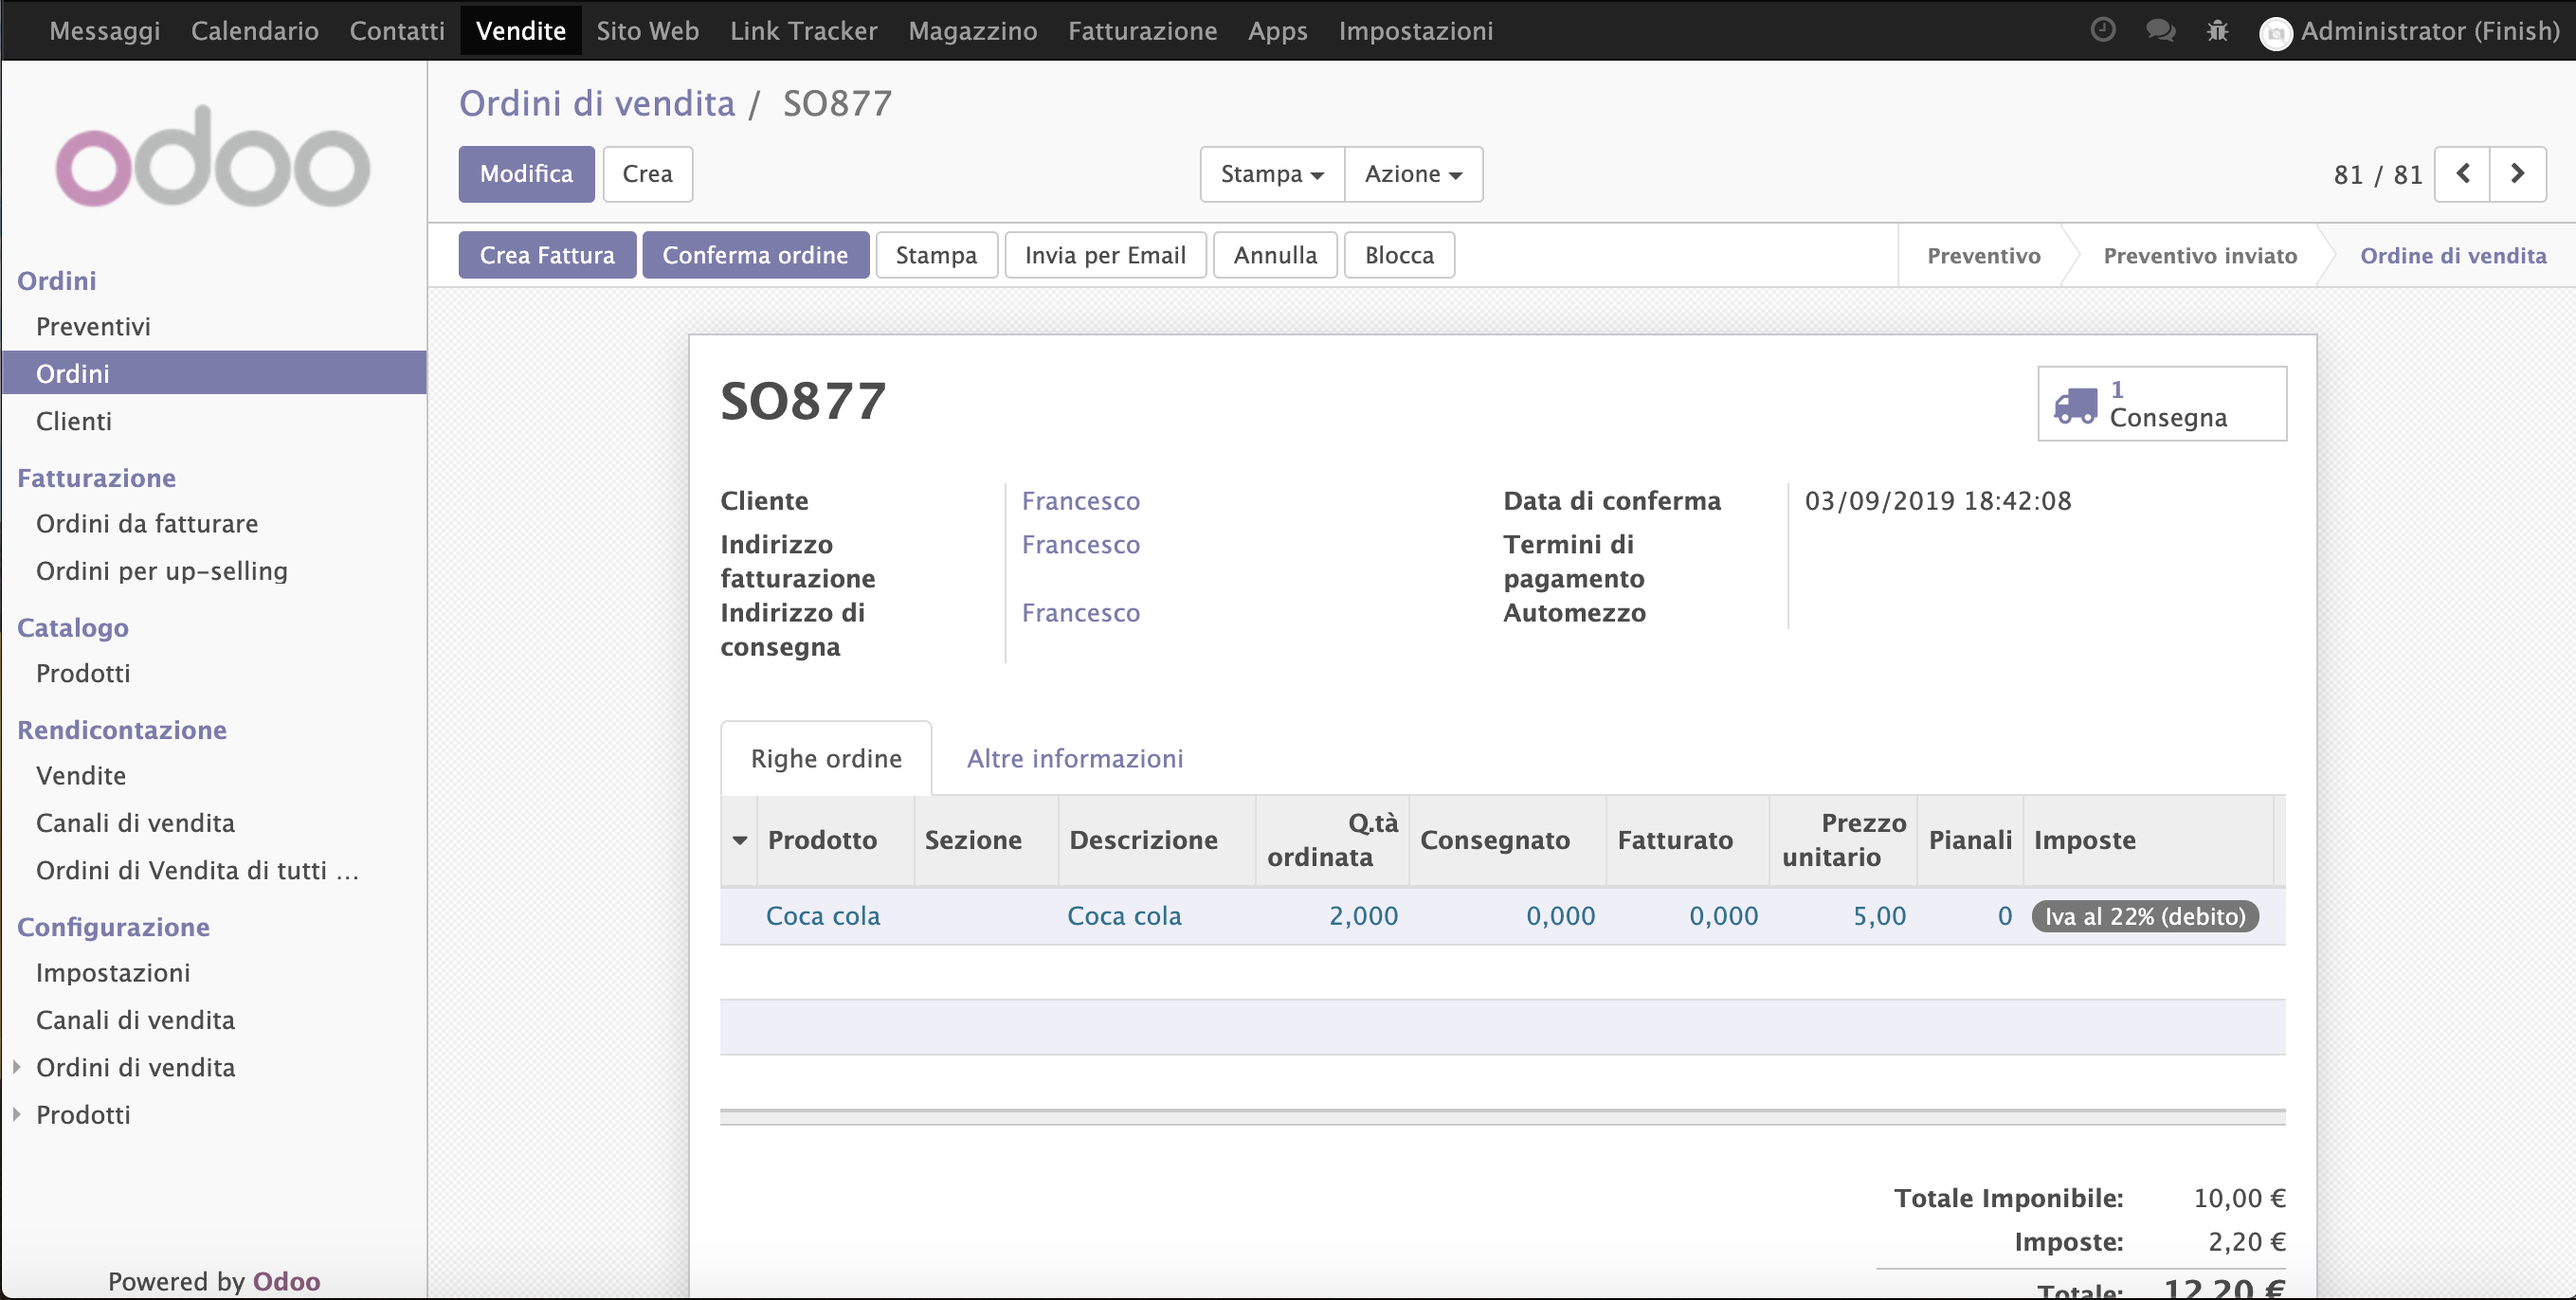
\includegraphics[scale=0.3]{figures/ctrl_test}
		\caption[Test sulle \textit{line} dei prodotti]{Test sulle \textit{line} dei prodotti}
		\label{fig:ctrl_test}
	\end{center}
\end{figure}
\newpage

\section{Test di Unità}

Per accertare la correttezza del codice as implemented dei modelli di ogni modulo si è ricorso ai test di \glo{unità}.
Sono stati svolti per verificare la funzione \textit{create}, cioè quella che crea, nuovi dati da salvare nel database per ogni singolo modulo.\\
Abbiamo testato tutti i modelli da me sviluppati.

\begin{figure}[H]
	\begin{center} 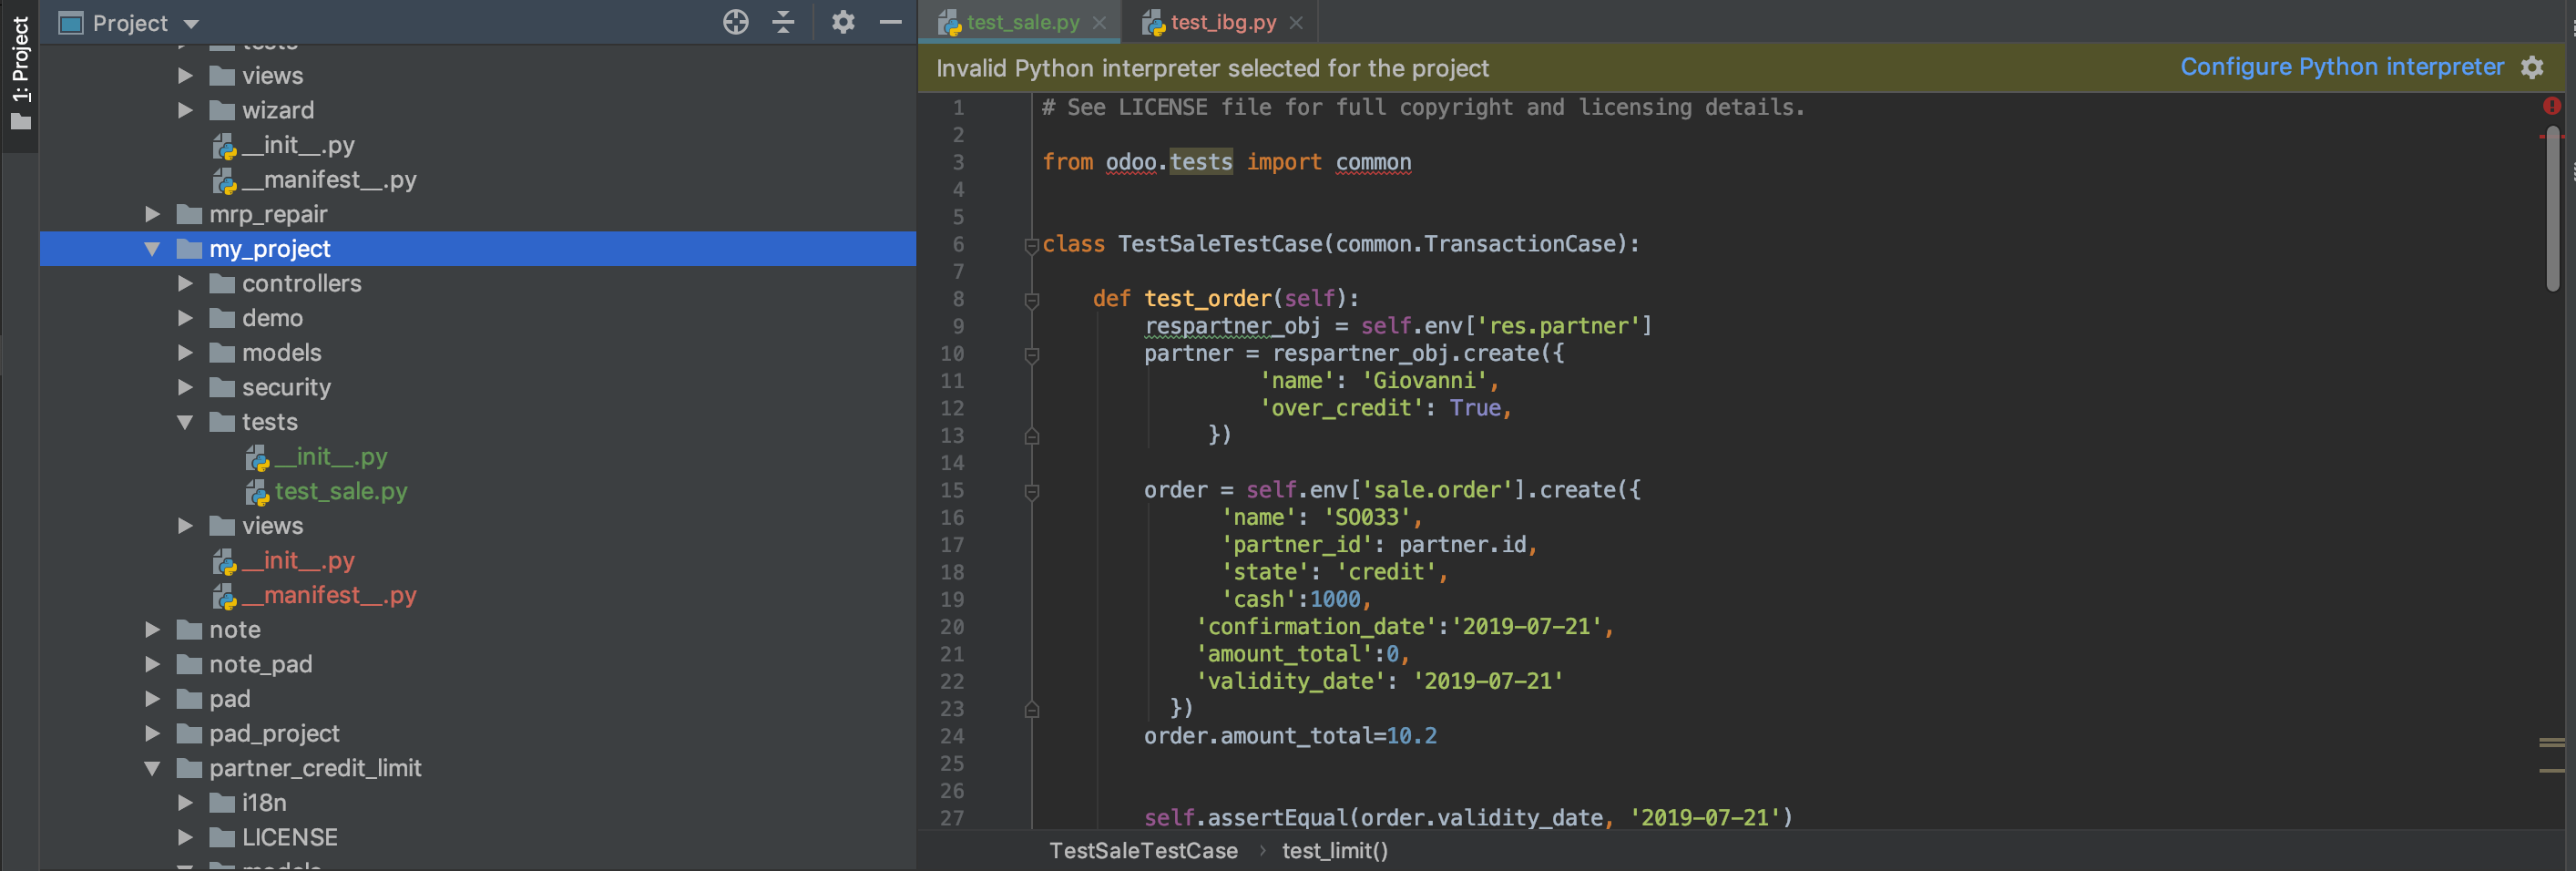
\includegraphics[scale=0.3]{figures/unit_test}
		\caption[Test di unità]{Test di unità}
		\label{fig:unit_test}
	\end{center}
\end{figure}
